\documentclass[10pt,conference,compsocconf]{IEEEtran}
\usepackage{datetime}
\usepackage{graphicx}
\usepackage{balance}
\usepackage{float}
\usepackage{xspace}
\usepackage[numbers,sort&compress,square]{natbib}
\usepackage{ctable}
%\makeatletter
%\renewcommand\bibsection%
%{
%  \section*{\refname
%    \@mkboth{\MakeUppercase{\refname}}{\MakeUppercase{\refname}}}
%}
%\makeatother

%\usepackage{times}
\usepackage{amsfonts}
\usepackage[cmex10]{amsmath}
\interdisplaylinepenalty=2500
\usepackage{amssymb}
\usepackage{dsfont}
\usepackage{mathtools}
\usepackage{graphicx}
\usepackage{subfig}
\usepackage{multirow}
\usepackage{bigstrut}
\usepackage{url}
\usepackage[ruled,linesnumbered]{algorithm2e}
\usepackage{mdwlist}


\DeclareCaptionType{copyrightbox}

\newtheorem{corol}{Corollary}
\newtheorem{conj}{Conjecture}
\newtheorem{lemma}{Lemma}
\newtheorem{claim}{Claim}
\newtheorem{theorem}{Theorem}

%\newdef{definition}{Definition}
\newtheorem{definition}{Definition}

\def\XXX{{\bf XXX}}
\def\MR{{\bf MR}}
\def\EK{{\bf EK}}

\def\betw{\mathsf{b}}
\def\kboundbetw{\mathsf{bb}}
\def\kpathbetw{\mathsf{pb}}
\def\prob{\pi}
\def\range{\mathcal{R}}
\def\TOPK{\mathsf{TOP}}
\def\VC{\mathsf{VC}}
\def\VD{\mathsf{VD}}

\begin{document}
\title{Fast Approximation of Betweenness Centrality Through Sampling}
\author{Submitted for blind review}
\maketitle

{\bf \large \today, \currenttime}

\ifdmkd
\else
\begin{abstract}
\fi
  %We present an efficient randomized algorithm for approximating the {\sl
  %betweenness centrality} of all nodes in a network within strict probabilistic
  %guarantees.
  Betweenness centrality is a fundamental measure in social network
  analysis, %, %quantifying
  expressing the importance or influence of individual vertices (or edges) in a
  network in terms of the fraction of shortest paths that pass through them. 
  %The fastest known algorithm to
  %compute the exact betweenness of all vertices in a graph $G=(V,E)$ in
  %$O(|V|\cdot|E|)$ steps in the unweighted case and in
  %$O(|V|\cdot|E|+|V|^2\log|V|)$ steps in weighted graphs. 
  Since exact computation in large networks %with millions of vertices and hundred of millions of edges 
  is prohibitively expensive, % and fast approximation algorithms are required in
  %these cases. 
  we present two efficient randomized %approximation 
  algorithms for betweenness
  estimation. The algorithms are based on random sampling of shortest paths and
  offer probabilistic guarantees on the quality of the approximation. 
  %One algorithm computes an $(\varepsilon,\delta)$-approximation of the vector
  %of betweenness centrality of all the vertices in the graph.
  The first algorithm estimates the betweenness of all vertices (or edges): all
  approximate values are within an additive factor $\varepsilon\in(0,1)$ from the real
  values, with probability at least $1-\delta$. The second algorithm focuses on
  the top-K vertices (or edges) with highest betweenness and estimate their betweenness
  value to within a multiplicative factor $\varepsilon$, with probability at least
  $1-\delta$. This is the first algorithm that can compute such approximation for
  the top-K vertices (or edges). 
  %We use results from the VC-dimension theory to develop
  %bounds to the sample size needed to achieve the desired approximations. 
  By proving upper and lower bounds to the VC-dimension of a range set
  associated with the problem at hand, we can bound the sample size needed to
  achieve the desired approximations. We obtain sample sizes that are
  independent from the number of vertices in the network and only depend on a
  characteristic quantity that we call the vertex-diameter, that is the maximum
  number of
  vertices in a shortest path. In some cases, the sample size is completely
  independent from any quantitative property of the graph.
  %Extensive experimental evaluation on real and artificial networks demonstrate
  %the practicality of our methods and their performances compared to exact and
  %approximated approximated algorithms.
  An extensive experimental evaluation on real and artificial networks shows
  that our algorithms are significantly faster and much more scalable as the
  number of vertices grows than other algorithms with similar approximation
  guarantees.
\ifdmkd
\else
\end{abstract}
\fi
  


\begin{IEEEkeywords}
betweenness centrality; sampling; social networks; VC-dimension;
\end{IEEEkeywords}

\section{Introduction}\label{sec:intro}
Centrality indices are fundamental metrics for network analysis. They express the
relative importance of a vertex in the network. Some of them, e.g., degree
centrality, reflect local properties of the underlying graph, while others,
like betweenness centrality, give information about the global network
structure, as they are based on shortest path computation and counting~\citep{Newman10}. In
this work we are interested in \emph{betweenness
centrality}~\citep{Anthonisse71,Freeman77}, that is, for every vertex in the
graph, the fraction of shortest paths that goes through that vertex (see
Section~\ref{sec:prelims} for formal definitions). Betweenness centrality has
been used to analyze social and protein networks, to evaluate traffic in
communication networks, and to identify important intersections in highway and
road networks~\citep{Newman10,GeisbergerSS08}. There exist polynomial-time
algorithms to compute the exact betweenness centrality~\citep{Brandes01}, but
they are not practical for the analysis of the very large networks that are of
interest these days. Graphs representing online social networks, communication
networks, and the web graph have millions of nodes and billions of edges,
making a polynomial-time algorithm too expensive in practice. Given that data
mining is exploratory in nature, approximate results are usually sufficient,
especially if the approximation error is guaranteed to be within user-specified
limits. In practice, the user is interested in the relative ranking of the
vertices according to their betweenness, rather than the actual value of the
betweenness, so a very good estimation of the value of each vertex is
sufficiently informative for most purposes. It is therefore natural to develop
algorithms that trade off accuracy for speed and efficiently compute
high-quality approximations of the betweenness of the vertices.  Nevertheless,
in order for these algorithms to be practical it is extremely important that
they scale well and have a low runtime dependency on the size of the network
(number of vertices and/or edges).

\paragraph{Our contributions} 
We present two randomized algorithms to approximate the betweenness centrality
(and some of its variants) of the vertices of a graph. The first algorithm
guarantees that the estimated betweenness values for all vertices are within an
\emph{additive} factor $\varepsilon$ from the real values, with probability at
least $1-\delta$. The second algorithm focuses on the top-$K$ vertices with
highest betweenness and returns a \emph{superset} of the top-$K$,
while ensuring that the estimated betweenness for all returned vertices is
within a \emph{multiplicative} factor $\varepsilon$ from the real value, with
probability at least $1-\delta$. This is the first algorithm to reach such a
high-quality approximation for the set of top-$K$ vertices. The algorithms are
based on random sampling of shortest paths. The analysis to derive the
sufficient sample size is novel and uses notions and results from VC-dimension
theory. We define a range set associated with the problem at hand and prove strict
upper and lower bounds to its VC-dimension. The resulting sample size \emph{does not
depend on the size of the graph}, but only on the maximum number of vertices
in a shortest path, a \emph{characteristic quantity} of the graph that we call
the \emph{vertex-diameter}. For some networks, we show that the VC-dimension is
actually
at most a constant and so the sample size depends \emph{only on the approximation
parameters} and not on any property of the graph, a somewhat surprising fact
that points out interesting insights. Thanks to the lower runtime dependency on
the size of the network, our algorithms are \emph{much faster and more scalable}
than previous contributions~\citep{JacobKLPT05,BrandesP07,GeisbergerSS08}, while
offering the same approximation guarantees. Moreover, the amount of work
performed by our algorithms per sample is also less than that of others algorithms.
We extensively evaluated our methods on real graphs and compared their
performances to the exact algorithm for betweenness centrality~\citep{Brandes01}
and to other sampling-based approximation
algorithms~\citep{JacobKLPT05,BrandesP07,GeisbergerSS08}, showing that our
methods achieve a huge speedup (3 to 4 times faster) and scale much better as
the number of vertices in the network grows.

We present related work in Sect.~\ref{sec:prevwork}. Section~\ref{sec:prelims}
introduces all the basic definitions and results that we will use throughout the
paper. A range set for the problem at hand and the bounds to its VC-dimension
are presented in Sect.~\ref{sec:rangeset}. Based on these results we develop and
analyze algorithms for betweenness estimation that we present in
Sect.~\ref{sec:algo}. Section~\ref{sec:exper} reports the methodology and
the results of our extensive experimental evaluation.


\section{Related work}\label{sec:prevwork}
Over the years, a number of centrality measures have been defined~\citep{Newman10}. In this work
we focus on betweenness centrality and some of its variants. 

Betweenness centrality was introduced in the sociology
literature~\citep{Anthonisse71,Freeman77} and many variants of it have been
developed over the year~\citet{Brandes08}. A particularly interesting variant
called ``$k$-bounded-distance betweenness'' limits the length of the shortest
paths considered when computing the
centrality~\citep{BorgattiE06,Brandes08,PfefferC12}. This is not to be confused
with ``$k$-path betweenness centrality''~\citet{KourtellisASIT12}, which
considers simple random walks that are not necessarily shortest paths.
\citet{DolevEP10} present a generalization of betweenness centrality which takes
into account routing policies in the network. \citet{OpsahlAS10} define a new
distance function between pair of vertices in order to penalize paths with a
high number of hops in weighted network. This function induces a generalized and
parametrized definition of betweenness.

The need of fast algorithms to compute the betweenness of vertices in a graph
arose as large online social networks started to appear. \citet{Brandes01} presents the
first efficient algorithm for the task, running in time $O(nm)$ on
unweighted graphs and $O(nm+n^2\log n)$ on weighted ones. The
algorithm computes, for each vertex $v$, the shortest path to every other vertex
and then traverses these paths backwards to efficiently compute the contribution
of the shortest paths from $v$ to the betweenness of other vertices. For very
large networks, the cost of this algorithm would still be prohibitive in
practice, so many approximation algorithms were
developed~\citep{JacobKLPT05,BrandesP07,BaderKMM07,GeisbergerSS08,MaiyaBW10,LimMRTB11}.
The use of random sampling was one of the more natural approaches to speed up
the computation of betweenness. Inspired by the work of~\citet{EppsteinW04},
\citet{JacobKLPT05} and independently \citet{BrandesP07} present an algorithm
that mimics the exact one, with the difference that,
instead of computing the contribution of all vertices to the betweenness of the
others, it only considers the contributions of some vertices sampled uniformly
at random. To guarantee that all estimates are within $\varepsilon$ from their
real value with probability at least $1-\delta$, the algorithm
from~\citep{JacobKLPT05,BrandesP07} needs $O(\log(n/\delta)/\varepsilon^2)$
samples. The analysis for the derivation of the sample size uses Hoeffding bounds~\citep{Hoeffding63} 
and the union bound~\citep{MitzenmacherU05}. 
\citet{GeisbergerSS08} noticed that this can lead
to an overestimation of the betweenness of vertices that are close to the
sampled ones and introduced different unbiased estimators that are
experimentally shown to have smaller variance and do not suffer from this
overestimation issue. Our algorithm takes a different approach from the above
algorithms. Specifically
it sample each time a single random shortest path. %between two randomly chosen nodes. 
This leads to a much smaller sample size and less work done for each sample,
resulting in a much faster way to compute approximations of the betweenness with
the same probabilistic guarantees. 
\ifproof
For certain applications it is sufficient to obtain a high-quality approximation
of the centrality of the top-K vertices. Although existing algorithms
\citep{BrandesP07,JacobKLPT05,GeisbergerSS08} can be extended to return a
superset of the top-$K$ vertices with highest betweenness, they only offer an
\emph{additive} approximation guarantee, while our algorithm for the top-$K$
vertices offers a \emph{multiplicative} factor guarantee, which is much
stricter. 
\fi
We delve more in the comparisons with these algorithms in
Sect.~\ref{sec:discussion} and~\ref{sec:exper}. 

A number of works explored
the use of adaptive sampling, in contrast with the previous algorithms (and
ours) which use a fixed sample size. \citet{BaderKMM07} present an adaptive
sampling algorithm which computes good estimations for the betweenness of
high-centrality vertices, by keeping track of the partial contribution of each
sampled vertex, obtained by performing a single-source shortest paths
computation to all other vertices. \citet{MaiyaBW10} use concepts from expander
graphs to select a connected sample of vertices. They estimate the betweenness
from the sample, which includes the vertices with high centrality. They build
the connected sample by adding the vertex which maximizes the number of
connections with vertices not already in the sample. Modified versions
of this algorithm and an extensive experimental evaluation appeared
in~\citep{LimMRTB11}. The algorithm does not offer any guarantee on the quality
of the approximations. Compared to these adaptive sampling approaches, our
methods ensure that the betweenness of all (or top-$K$) vertices is well
approximated, while using a fixed, predetermined amount of samples.
\citet{SaryuceSKC13} present an algorithm that pre-processes the network in
multiple ways by removing degree-1 vertices and identical vertices and splitting
the network" in separate components where the computation of betweenness can be
performed independently and then aggregated. They do not present an analysis of
the complexity of the algorithm. 

In the analysis of our algorithm we use results from VC-dimension
theory~\citep{VapnikC71}, a key component of statistical learning theory. We
compute an upper bound to the VC-dimension of a range set defined on shortest
paths. \citet{KranakisKRUW97} present a number of results on the VC-dimension of
various range sets for graphs (stars, connected sets of vertices, sets of
edges), but do not study the case of shortest paths. \citet{AbrahamDFGW11} use
VC-dimension to speed up shortest path computation but their range set is
different from the one we use: their ground set is the set of vertices while
ours is defined on shortest paths.

\ifproof
The present work extends substantially the preliminary
version~\citep{RiondatoK14WSDM}. The proof of all the theorems and lemmas are
presented here for the first time. Examples of betweenness centrality and of the
concept of VC-dimension have been added to Sect.~\ref{sec:prelims}. A major new
contribution is a tighter analysis of the algorithm from~\citep{BrandesP07} and
a thorough comparison with it, presented in Sect.~\ref{sec:discussion}. We also
discuss many other variants of betweenness, including edge betweenness in
Sect.~\ref{sec:variants}, where we also present a new tighter analysis of the
algorithm for $k$-path betweenness centrality by~\citep{KourtellisASIT12}.  %An expanded
%motivation for the top-$k$ algorithm opens Sect.~\ref{sec:topk}. 
%Finally, we report many additional
%results of our experimental evaluation, including results on the top-$k$
%algorithm, in Sect.~\ref{sec:exper}.
\fi


\section{Preliminaries}\label{sec:prelims}
In this section we introduce the definitions and lemmas that we will use to
develop and analyze our results in the remainder of the paper.

\subsection{Graphs and betweenness centrality}\label{sec:graphprelims}
Let $G=(V,E)$ be a graph, where $E\subseteq V\times V$, with $n=|V|$ vertices
and $m=|E|$ edges. Each edge
$e\in E$ has a positive weight $\mathsf{w}(e)$. The graph
$G$ can be directed or undirected. We assume
that there are no self-loops and no multiple edges between a pair of vertices.
Given a pair of vertices $(u,v)\in V\times V$,
$u\neq v$, a \emph{path $p_{uv}\subseteq V$ from $u$ to $v$} is an ordered sequence of
vertices $p_{uv}=(w_1,\dotsc,w_{|p_{uv}|})$ such that $w_1=u$, $w_{|p_{uv}|}=v$ and
for each $1\le i < |p_{uv}|$, $(w_i,w_{i+1})\in E$. The vertices $u$ and $v$ are
called the \emph{end points} of $p_{uv}$ and the vertices in
$\mathsf{Int}(p_{uv})=p_{uv}\setminus\{u,v\}$ are the \emph{internal vertices of
$p_{uv}$}. The \emph{weight}
$\mathsf{w}(p_{uv})$ of a path $p_{uv}=(u=v_1,v_2,\cdots,v_{p_{|uv|}}=v)$ from
$u$ to $v$ is the sum of the weights of the edges composing the path:
$\mathsf{w}(p_{uv})=\sum_{i=1}^{|p_{uv}|-1}\mathsf{w}((v_i,v_{i+1}))$. We denote with
$|p_{uv}|$ the number of vertices composing the path and call this the
\emph{size of the path $p_{uv}$}. Note that if the weights are not all unitary,
it is not necessarily true that $\ell(p_{uv})=|p_{uv}|-1$. A special and
degenerate path is the \emph{empty path} $p_{\emptyset}=\emptyset$, which by
definition has weight $\mathsf{w}(p_\emptyset)=0$, no end points, and
$\mathsf{Int}(p_\emptyset)=\emptyset$.

Given two distinct vertices $(u,v)\in V\times V$, the \emph{shortest path distance}
$d_{uv}$ between $u$ and $v$ is the weight of a path with minimum weight 
between $u$ and $v$, among all paths between $u$ and $v$. If there is no path
between $u$ and $v$, $d_{uv}=0$. We call a path between $u$ and $v$ with
weight $d_{uv}$ a \emph{shortest path between $u$ and $v$}. There can be
multiple shortest paths between $u$ and $v$ and we denote the set of these paths
as $\mathcal{S}_{uv}$. If there is no path between $u$ and $v$, then
$\mathcal{S}_{uv}=\{p_\emptyset\}$\footnote{Note that even if
$p_\emptyset=\emptyset$, the set $\{p_\emptyset\}$ is not empty. It contains
one element.}.
%By definition, $\mathcal{S}_{vv}=\emptyset$.
We denote with $\mathbb{S}_G$ the union of all the $\mathcal{S}_{uv}$'s, for all
pair $(u,v)\in V\times V$ of distinct nodes $u\neq v$: 
\[ \mathbb{S}_G=\bigcup_{\substack{(u,v)\in V\times V \\ u\neq v}}\mathcal{S}_{uv}\enspace.\]

We now define a characteristic quantity of a graph that we will use throughout
the paper.
\begin{definition}\label{def:vertexdiam}
  Given a graph $G=(V,E)$, the \emph{vertex-diameter $\VD(G)$ of $G$} is the
  maximum size of a shortest path between a pair of vertices of $V$:
  \[
  \VD(G) = \max\left\{|p| ~:~ p\in \mathbb{S}_G\right\}\enspace.\]
\end{definition}
If all the edge weights are unitary, then $\VD(G)$ is equal to
$\mathsf{diam}(G)+1$, where $\mathsf{diam}(G)$ is the number of edges composing the
longest shortest path in $G$.
Given a vertex $v$, let $\mathcal{T}_v\subseteq\mathbb{S}_G$ be the set of all
shortest paths that $v$ is \emph{internal} to:
\[
\mathcal{T}_v=\{p\in\mathbb{S}_G ~:~ v\in\mathsf{Int}(p)\}\enspace.
\]
In this work we are interested in the \emph{betweenness centrality} of the
vertices of a graph.
\begin{definition}[\citep{Anthonisse71,Freeman77}]\label{def:betwenness}
  Given a graph $G=(V,E)$, the \emph{betweenness centrality of a vertex $v\in
  V$} is defined as
  \[
  \betw(v)=\frac{1}{n(n-1)}\sum_{p_{uw}\in\mathbb{S}_G}\frac{\mathds{1}_{\mathcal{T}_v}(p)}{|\mathcal{S}_{uw}|}=\frac{1}{n(n-1)}\sum_{p_{uw}\in\mathcal{T}_v}\frac{1}{|\mathcal{S}_{uw}|}\enspace.
  \]
\end{definition} 

It is easy to see that $\betw(v)\in[0,1]$.\footnote{We use the normalized
version of betweenness as we believe it to be more suitable for presenting approximation
results.} \citet{Brandes01} presented an
algorithm to compute the betweenness centrality for all $v\in V$ in time
$O(nm)$ for unweighted graphs and $O(nm + n^2 \log n)$ for weighted graphs. 

A ``local'' variant of betweenness, called \emph{$k$-betweenness} only considers
the contribution of paths of size up to $k+1$~\citep{BorgattiE06,Brandes08}.
For $k>1$ and any pair of distinct vertices $u,v\in V$, $u\neq V$, let
$\mathcal{S}^{(k)}_{uv}\subseteq\mathcal{S}_{uv}$ be the set of shortest paths
from $u$ to $v$ of size at most $k+1$, and let $\mathbb{S}^{(k)}_G$ be the union
of all the $\mathcal{S}^{(k)}_{uv}$. Let
$\mathcal{T}^{(k)}_v\subseteq\mathcal{T}_v$ be the set of all shortest paths
\emph{of size up to $k$} that $v$ is internal to, for each $v\in V$.

\begin{definition}[\citep{BorgattiE06,Brandes08}]\label{def:kbetweenness}
 
  Given a graph $G=(V,E)$ and an integer $k>1$, the \emph{$k$-betweenness
  centrality of a vertex $v\in V$} is defined as
  \[
  %\betw(v)=\sum_{(u,w)\in V\times
  %V}\sum_{p\in\mathcal{S}_{uw}}\frac{\mathds{1}_{\mathcal{T}_v}(p)}{|\mathcal{S}_{uw}|}\enspace.
  %\betw(v)=\sum_{p_{uw}\in\mathbb{S}_G}\frac{\mathds{1}_{\mathcal{T}_v}(p)}{|\mathcal{S}_{uw}|}\enspace.
  \betw^{(k)}(v)=\frac{1}{n(n-1)}\sum_{p_{uw}\in\mathbb{S}^{(k)}_G}\frac{\mathds{1}_{\mathcal{T}^{(k)}_v}(p)}{\left|\mathcal{S}^{(k)}_{uw}\right|}=\frac{1}{n(n-1)}\sum_{p_{uw}\in\mathcal{T}^{(k)}_v}\frac{1}{\left|\mathcal{S}^{(k)}_{uw}\right|}\enspace.
  \]
\end{definition}

Another interesting variant of betweenness centrality do not consider
\emph{shortest} paths, but rather \emph{simple random walks} of size up to
$k+1$, expressing the intuition that information in a network does not
necessarily spread across shortest paths but has a high probability of ``fading
out'' after having touched at most a fixed number of vertices.

\begin{definition}[\citep{KourtellisASIT12}]\label{def:kpathbetweenness}
 Given a graph $G=(V,E)$ and a positive integer $k$, the \emph{$k$-path
 centrality} Ck(v) of $v\in V$ is defined as the average\footnote{We take the
 average, rather than the sum, as defined in the original work
 by~\citet{KourtellisASIT12}, to normalize the value to fall in the interval
 $[0,1]$}, over all possible source
 nodes $s$, of the probability that a simple random walk originating from
 $s$ and extinguishing after having touched (at most) $k+1$ vertices ($s$
 included) goes through $v$.
\end{definition}

\citet{KourtellisASIT12} present a randomized approximation algorithm to
estimate, with probability at least $1-1/n^2$, all the $k$-path betweenness
values to within an additive error $n^{-1/2+\alpha}$ in time
$O(k^3n^{2-2\alpha}\ln n)$.

\subsection{Vapnik-Chervonenkis dimension}\label{sec:prelvcdim}
The Vapnik-Chernovenkis (VC) dimension of a class of subsets defined
on a set of points is a measure of the complexity or expressiveness of such
class~\citep{VapnikC71}. Given a probability distribution on the set of points,
a finite bound on the VC-dimension of the class of subsets implies a bound on
the number of random samples required to approximate the probability of each
subsets its empirical average. We outline here some basic definitions and
results and refer the reader to the book of~\citet{MohriRT12} for an in-depth
presentation.
%works of~\citet[Sect.~14.4]{AlonS08} and
%\citet[Sect.~3]{BoucheronBL05} for an introduction of VC-dimension and a survey
%of recent developments. \XXX Cite book Foundations of ML instead.
%~\citet[Sect.~12.4]{DevroyeGL96},
%\citet[Sect.~3]{BoucheronBL05}, \citet[Sect.~14.4]{AlonS08}, and
%\citet{Vapnik99} for more details on VC-dimension.

Let $D$ be a domain and $\range$ be a collection of subsets from $D$. We call
$\range$ a \emph{range set on $D$}.
Given $B\subseteq D$, the \emph{projection of $\range$ on $B$} is the set 
$P_\range(B)=\{ B\cap A ~:~ A\in\range\}$. We say that the set $B$ is
\emph{shattered} by $\range$ if $P_\range(B)=2^B$.

\begin{definition}\label{def:vcdim}
  The \emph{Vapnik-Chervonenkis (VC) dimension of $\range$}, denoted as
  $\VC(\range)$, is the cardinality of the largest subset of $D$ that is
  shattered by $\range$.
\end{definition}

The main application of VC-dimension in statistics and learning
theory is in computing the number of samples needed to approximate the
probabilities associated to the ranges through their empirical averages.
Formally, let $X_1^k=(X_1,\dotsc,X_k)$ be a collection of independent
identically distributed random variables taking values in $D$, sampled 
according to some distribution $\phi$ on the elements of $D$.
For a set $A\subseteq D$, let $\phi(A)$ be the probability that a sample from
$\phi$ belongs to the set $A$, and let
\[
\phi_{X_1^k}(A)=\frac{1}{k}\sum_{j=1}^k\mathds{1}_A(X_j)\enspace.%, 
\]
%where $\mathds{1}_A$ is the indicator function for the set $A$. 
The function
$\phi_{X_1^k}(A)$ is the \emph{empirical average} of $\phi(A)$ on $X_1^k$.

\begin{definition}\label{def:eapprox}
  Let $\range$ be a range set on %a domain
  $D$ and $\phi$ be a probability distribution on $D$. For $\varepsilon\in(0,1)$,
  an \emph{$\varepsilon$-approximation to $(\range,\phi)$} is a bag $S$ of
  elements of $D$ such that 
  \[
  \sup_{A\in\range}|\phi(A)-\phi_S(A)|\le\varepsilon\enspace.\]
\end{definition}

An $\varepsilon$-approximation can be constructed by sampling points of
the domain according to the distribution $\phi$, provided an upper bound to the
VC-dimension of $\range$:

\begin{theorem}[Thm.~2.12~\citep{HarPS11}]\label{thm:eapprox}
  (see also~\citep{LiLS01}). Let $\range$ be a range set on a domain $D$ with
  $\VC(\range)\le d$, and let $\phi$ be a distribution on $D$. Given
  $\varepsilon,\delta\in(0,1)$ let $S$ be a collection of $|S|$ points from $D$
  sampled according to $\phi$ for
  \begin{equation}\label{eq:vceapprox}
	|S|=\frac{c}{\varepsilon^2}\left(d+\ln\frac{1}{\delta}\right)
  \end{equation}
  where $c$ is an universal positive constant. Then, $S$ is an
  $\varepsilon$-approximation to $(\range,\phi)$ with probability at least
  $1-\delta$.
\end{theorem}
\citet{LofflerP09} showed experimentally that the constant $c$ is approximately
$0.5$. We used this value in our experiments.

A similar definition offers relative guarantees on the approximation.
\begin{definition}\label{def:releapprox}
  Let $\range$ be a range set on $D$ and $\phi$ be a probability distribution on
  $D$. For $\epsilon,pi\in (0,1)$, a \emph{relative
  $(p,\varepsilon)$-approximation to $(\range,\phi)$} is a bag $S$ of elements
  from $D$ such that 
  \begin{itemize}
    \item For any $A\in\range$ such that $\phi(A)\ge p$, we have 
      \[ |\phi(A) - \phi_S(A)|\le \varepsilon\phi(A)\enspace.\]
    \item For any $B\in\range$ such that $\phi(B)< p$, we have $\phi_S(B)\le
      (1+\varepsilon)p$.
  \end{itemize}
\end{definition}

\begin{theorem}[Thm.~2.11~\citep{HarPS11}]\label{thm:releapprox}
  Let $\range$ be a range set on a domain $D$ with
  $\VC(\range)\le d$, and let $\phi$ be a distribution on $D$. Given
  $\varepsilon,\delta,p\in(0,1)$ let $S$ be a collection of $|S|$ points from $D$
  sampled according to $\phi$ for
  \begin{equation}\label{eq:releapprox}
    |S|\ge\frac{c'}{\varepsilon^2p}\left(d\log\frac{1}{p}+\log\frac{1}{\delta}\right)
  \end{equation}
  where $c'$ is an absolute positive constant. Then $S$ is a relative
  $(p,\varepsilon$-approximation to $(\range,\phi)$ with probability at least
  $1-\delta$.
\end{theorem}


\section{A range set of shortest paths}\label{sec:rangeset}
We now define a range set of the shortest paths of a graph $G=(V,E)$, and present 
an upper bound to its VC-dimension. We show that this upper bound is strict. We
use the range set and the bound in the analysis of our algorithm for estimating
the betweenness centrality of vertices of $G$.

The range set $\range_G$ is defined on the set $\mathbb{S}_G$ of all shortest
paths between vertices of $G$. It contains, for each vertex $v\in V$, the set
$\mathcal{T}_v$ of shortest paths that $v$ is internal to:
\[
\range_G = \{\mathcal{T}_v ~:~ v\in V\}\enspace.
\]

\begin{lemma}\label{lem:vcdimuppbound}
  %Given a graph $G=(V,E)$ with vertex-diameter $\Delta_G$, the range set
  %$\range_G$ associated to the shortest paths in $G$ has VC-dimension
  $\VC(\range_G)\le\lfloor\log_2(\VD(G)-2)\rfloor+1$.
\end{lemma}

\begin{proof}
%\begin{IEEEproof}
Let $\ell>\lfloor\log_2(\VD(G)-2)\rfloor+1$ and assume for the sake of contradiction
that $\VC(\range_G)=\ell$. From the definition of the VC-dimension there is a set
$Q\subseteq\mathbb{S}_G$ of size $\ell$ that is shattered by $\range_G$. Let $p$ be
an element of $Q$. There are  $2^{\ell-1}$ non-empty subsets of
$Q$ containing the path $p$. Let us label these non-empty subsets of $Q$ containing $p$ as
$S_1,\dotsc,S_{2^{\ell-1}}$, where the labelling is arbitrary.
Given that $Q$ is shattered then, for each set $S_i$ there must be a range $R_i$ in
$\range_G$ such that $S_i=Q\cap R_i$. Since all the $S_i$'s are
different from each other, then all the $R_i$'s must be different from each
other. Given that $p$ belongs to each $S_i$, then $p$ must also belong to each
$R_i$, that is, there are $2^{\ell-1}$ distinct ranges in $\range_G$ containing
$p$. But $p$ belongs only to the ranges corresponding to the internal vertices of
$p$, i.e., to the vertices in $\mathsf{Int}(p)$. This means that the number of ranges
in $\range_G$ that $p$ belongs to is equal to $|p|-2$. But $|p|\le\VD(G)$, by
definition of $\VD(G)$, so $p$
can belong to at most $\VD(G)-2$ ranges from $\range_G$. Given that
$2^{\ell-1}>\VD(G)-2$, we reached a contradiction and there cannot be $2^{\ell-1}$
distinct ranges containing $p$, hence not all the sets $S_i$ can be expressed as
$Q\cap R_i$ for some $R_i\in\range_G$, but then $Q$ cannot be shattered and
$\VC(\range_G)\le\lfloor\log_2(\VD(G)-2)\rfloor+1$.%\qed
\end{proof}
%\end{IEEEproof}

\paragraph{Unique shortest paths}\label{sec:rangeunique}
\XXX I really need to check whether this is only for undirected case

In the restricted case when %the graph is undirected and
every pair of distinct vertices has either none or a unique shortest path
between them, the VC-dimension of $\range_G$ collapses to a \emph{constant}. This is a
somewhat surprising result with interesting consequences. From a theoretical
point of view, it suggests out that there sohuld be other characteristic
quantities of the graph different from the vertex diameter that control the
VC-dimension of the range set of shortest paths, and these quantities are
constant on graph with unique shortest paths between vertices. From a more
practical point of view, we will see in Sect.~\ref{sec:algo} that this result has an
impact on the sample size needed for approximating the betweenness centrality of
networks where the unique-shortest-path property is satisfied or even enforced,
like road networks~\citep{GeisbergerSS08}. In particular, the resulting sample
size will be \emph{completely independent} from any characteristic of the
network, and will only be a function of the parameters controlling the desired
approximation guarantees.

\begin{lemma}\label{lem:vcdimuppboundunique}
  Given a %n undirected
  graph $G=(V,E)$ such that $|\mathcal{S}_{uv}|\le1$ for all
  pairs $(u,v)\in V\times V$, the range set $\range_G$ associated to the
  shortest paths in $G$ has VC-Dimension $\VC(\range_G)\le3$.
\end{lemma}

\begin{proof}
%\begin{IEEEproof}
  First of all, notice that in this restricted setting, if two different
  shortest paths $p_1$ and $p_2$ meet at a vertex $u$, then they either go on
  together or at a certain point they separate never to meet again at any other
  vertex $v\neq u$.  This is easy to see: if they could separate and then meet
  again, then there would be two distinct shortest paths between $u$ and $v$,
  which is a contradiction of the hypothesis. Let us denote this fact as
  $\mathsf{F}$.

  Assume now that $\VC(\range_G)>3$, then there must be a set
  $Q=\{p_1,p_2,p_3,p_4\}$ of four shortest paths that can be shattered by
  $\range_G$. Then there is a vertex $w$ such that $\mathcal{T}_w\cap Q=Q$, i.e.,
  all paths in $Q$ go through $w$. Let $x$ be the farthest predecessor of $w$
  along $p_1$ that $p_1$ shares with some other path from $Q$, and let $y$ be
  the farthest successor of $w$ along $p_1$ that $p_1$ shares with some other
  path from $Q$. It is easy to see that if either $x$ or $y$ (or both) do not
  exist, then $Q$ cannot be shattered, as we would incur in a contradiction of
  $\mathsf{F}$. Let us then assume that both $x$ and $y$ exist.
  Let $Q_x=\mathcal{T}_x\cap Q$ and $Q_y=\mathcal{T}_y\cap Q$.
  Because of fact $\mathsf{F}$, all paths in $Q_x$ must go through the same vertices
  between $x$ and $w$ and all paths in $Q_y$ must go through the same vertices
  between $w$ and $y$. This also means that all paths in $Q_x\cap Q_y$ must go
  through the same vertices between $x$ and $y$. If $Q_x\cup Q_y\neq Q$, let
  $p^*\in Q\setminus(Q_x\cup Q_y)$ then from the definition of $x$ and $y$ and
  from fact $\mathsf{F}$ we have that there is no vertex $v$ such that
  $\mathcal{T}_v\cap Q=\{p_1,p^*\}$, which implies that $Q$ can not be
  shattered. Suppose from now on that $Q_x\cup Q_y=Q$.  If $Q_x\cap Q_y=Q$, then
  all the paths in $Q$ go through the same vertices between $x$ and $y$. From
  this and the definition of $x$ and $y$ we have that there is no vertex $v$
  such that, for example, $\mathcal{T}_v\cap Q=\{p_1,p_2\}$, hence $Q$ cannot be
  shattered. Suppose instead that $Q_x\cap Q_y\neq Q$ and let $S=(Q_x\cap
  Q_y)\setminus\{p_1\}$. If $S\neq\emptyset$ then there is at least a path
  $p'\in S$ which, from the definition of $S$ and fact $\mathsf{F}$, must go
  through all the same vertices as $p_1$ between $x$ and $y$. Moreover, given
  that $Q_x\cap Q_y\neq Q$, there must be a path $p^*\in Q\setminus\{p_1\}$
  different from $p_1$ such that $p^*\notin S$. Then, from the definition of
  $x$, $y$, and $S$, and from the existence of $p'$, there can be no vertex $v$
  such that $\mathcal{T}_v\cap Q=\{p_1,p^*\}$, hence $Q$ cannot be shattered.
  Assume now that $S=\emptyset$ and consider the case $Q_x=\{p_1,p_2,p_3\}$,
  $Q_y=\{p_1,p_4\}$ (all other cases follow by symmetry with this case).
  Consider the set $\{p_1,p_3\}$. From the definition of $x$ and $Q_x$, and from
  fact $\mathsf{F}$ we have that there can not be a vertex $v$ between the end
  point of $p_1$ before $x$ and $w$ such that $\mathcal{T}_v\cap Q=\{p_1,p_3\}$.
  At the same time, from the definition of $y$ and from fact $\mathsf{F}$, we
  have that such a $v$ can not be between $w$ and the end point of $p_1$ after
  $y$. This implies that $Q$ can not be shattered.

  We showed that in all possible cases we reached a contradiction and $Q$,
  which has size $4$, can not be shattered by $\range_G$. Hence $\VC(\range_G)\le
  3$.
%\end{IEEEproof}
\end{proof}

%\subsection{Variants}\label{sec:rangevariants}
\paragraph{Bounded-distance betweenness}
For the case of $k$-bounded-distance betweenness, if we let
$\range_G^{(k)}=\{\mathcal{T}_v^{(k)}~:~ v\in V\}$, it is easy to bound
$\VC(\range_G^{(k)})$ following the same reasoning as in
Lemma~\ref{lem:vcdimuppbound}.
\begin{lemma}\label{lem:vcdimuppboundk}
$\VC(\range_G^{(k)})\le\lfloor\log_2(k-1)\rfloor+1$.
\end{lemma}

%\paragraph{$k$-path betweenness} We can define another range set
%$\range_G^{\mathrm{p},k}$ if we are interested in $k$-path betweenness. The
%domain $B$ of the range set now is the set of all simple random walks starting
%from any vertex of and of size up to $k+1$. For each vertex $v\in V$, the range
%$R_v$ is the subset of $B$ containing all and only the random walks from $B$
%that have $v$ as internal vertex. It is easy to see that
%$\VC(\range_G^{\mathrm{p},k})$ is still at most $\lfloor\log_2(k-1)+1$
%following the same reasoning as in Lemma~\ref{lem:vcdimuppbound}.

\subsection{Tightness}\label{sec:tightness}
The bound presented in Lemma~\ref{lem:vcdimuppbound} is strict in the sense that
for each $d\ge 1$ we can build a graph $G_d$ with vertex-diameter
$\VD(G_d)=2^d+1$ and such that the range set $\range_{G_d}$ associated to the set of
shortest paths of $G_d$ has VC-dimension exactly
$d=\lfloor\log_2(\VD(G_d)-2)\rfloor+1$. For the sake of clarity, we will discuss
only the case of undirected graphs with equal edge weights, but all we say can
be easily adapted to the general case.

We now introduce a class $\mathcal{G}=(G_d)_{d\ge 1}$ of graphs indexed by $d$.
The graphs in $\mathcal{G}$ are the ones for which we can show the tightness of
the bound to the VC-dimension of the associated range set.
We call the graph $G_d\in\mathcal{G}$ the \emph{$d$-th concertina graph}.
Figure~\ref{fig:tightgraphs} shows $G_1$, $G_2$, $G_3$, and $G_4$. The
generalization to higher values of $d$ should be straightforward.
By construction, $\VD(G_d)=2^d+1$, so that
$\lfloor\log_2(\VD(G_d)-2)\rfloor+1=d$. The $3(2^{d-1})$ vertices of $G_d$ can
be partitioned into three classes, \emph{top}, \emph{bottom}, and \emph{middle},
according to their location in a drawing of the graph similar to that in
Fig.~\ref{fig:tightgraphs}. $G_d$ $2^{d-1}-1$ top vertices, $2^{d-1}-1$ bottom vertices, and
$2^{d-1}+2$ middle vertices. For each top vertex $v$, let $\mathsf{f}(v)$ be the
\emph{corresponding bottom vertex}, i.e., the bottom vertex $u$ whose neighbors
are the same middle vertices that are neighbors of $v$. Among the middle
vertices, the two with degree 1 are special and are called the \emph{end
vertices} of $G_d$ and denoted as $v_\ell$ and $v_\mathrm{r}$, where the
labels can be arbitrarily assigned. We are now going to build a set $Q$ of $d$
shortest paths from $v_\ell$ to $v_\mathrm{r}$ and show that it is
shattered by $\range_{G_d}$, therefore proving that $\VC(\range_{G_d})\ge d$.
This fact, together with Lemma~\ref{lem:vcdimuppbound}, allows us to conclude
that $\VC(\range_{G_d})=d$. 

\begin{figure}[ht]
  \centering
  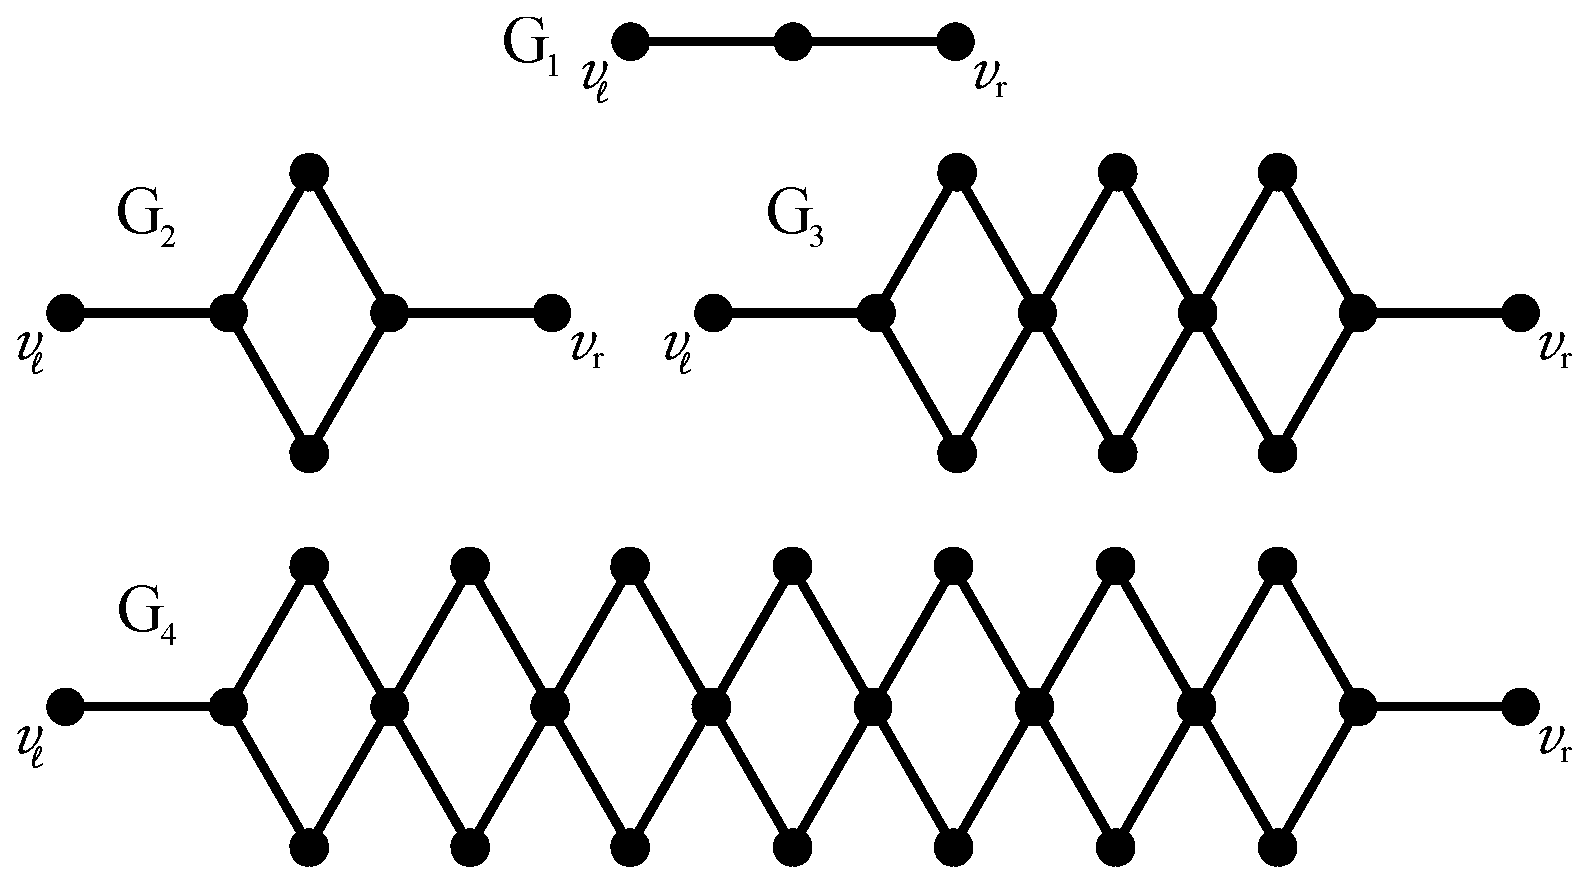
\includegraphics[scale=0.3]{tight}
  \caption{Examples of concertina graphs $G_d$ for $d=1,2,3,4$.}
  \label{fig:tightgraphs}
\end{figure}

\begin{lemma}\label{lem:vcdimlowbound}
  $\VC(\range_{G_d})=d$.
\end{lemma}

\begin{proof}
%\begin{IEEEproof}
  As we said, the $d$ paths in $Q$  go from $v_\ell$ to $v_\mathrm{r}$.
  From this and the definition of $G_d$ it should be clear that they must go through
  all the middle vertices of $G_d$. Consider now the set
  $S=2^Q\setminus\{Q,\emptyset\}$. We are now going to build a map $\mathsf{r}$
  from the elements of $S$ to the set of top and bottom vertices of $G_d$ We can
  partition $S$ in two sets $A$ and $B$ such that $A\cap B=\emptyset$ and $A\cup
  B=Q$ in the following way: for each unordered pair $(s',s'')$ of
  elements in $S$ such that $s'\cap s''=\emptyset$ and $s'\cup s''=Q$
  we put $s'$ in $A$ and $s''$ in $B$. The map $\mathsf{r}$ will map the
  elements of $A$ to the top vertices of $G_d$ and the elements of $B$ to the
  bottom vertices. For each $s'\in A$, let $\mathsf{c}(s')$ be the element $s''$
  of $B$ such that $s'\cap s''=\emptyset$ and $s'\cup s''=Q$. It is
  easy to see that the size of $A$ ($|A|=2^{d-1}-1$) equals the number of top
  vertices of $G_d$, and analogously for $B$ and the number of bottom vertices.
  Let $\mathsf{r}_A$ be an arbitrary one-to-one map from the elements of $A$ to
  the top vertices of $G_d$. Consider now the inverse map $\mathsf{r}^{-1}_A$
  from the top vertices to the elements of $A$. We can create another map
  $\mathsf{r}_B$ from $B$ to the
  bottom vertices of $G_d$ that maps the element
  $\mathsf{c}(\mathsf{r}^{-1}_A(v))$ of $B$ to the bottom vertex $\mathsf{f}(v)$
  corresponding to $v$, for each top vertex $v$. A path $p\in Q$ goes through
  a top vertex $v$ if and only if $p\in\mathsf{r}^{-1}_A(v)$. Analogously, $p$
  goes through a bottom vertex $u$ if and only if $p\in\mathsf{r}^{-1}_B(u)$.
  It is easy to see that, if we combine $\mathsf{r}_A$ and
  $\mathsf{r}_B$, we obtain a map $\mathsf{r}$ from $S$ to the set of
  top and bottom vertices of $G_d$. An example of a possible $\mathsf{r}$ for
  $G_3$ is presented in Fig.~\ref{fig:mapexample}.

  \begin{figure}[ht]
    \centering
    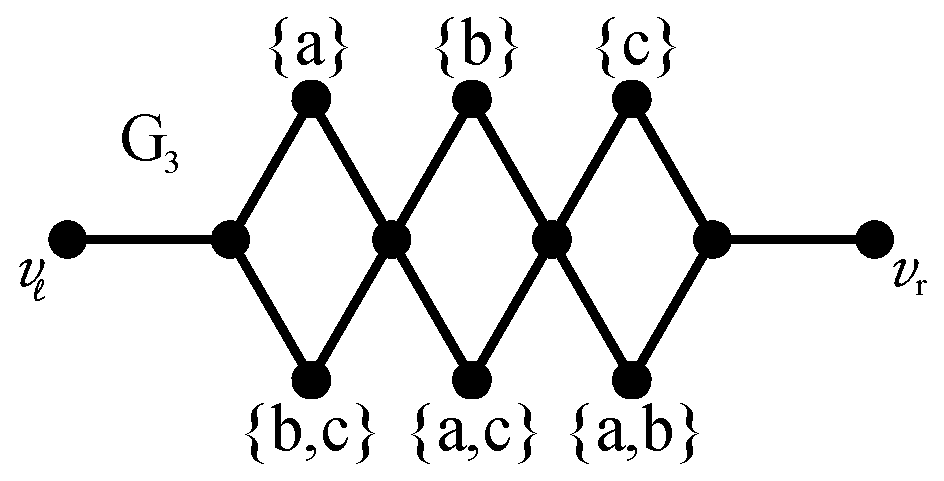
\includegraphics[scale=0.4]{tight-mapexample}
    \caption{An example of the $\mathsf{r}$ map for $G_3$. The set next to
    each top and bottom vertex $u$ is the set $s$ such that $\mathsf{r}(s)=u$.}
    \label{fig:mapexample}
  \end{figure}
  
  We now show that for each $s\in S$, $s=Q\cap\mathcal{T}_{\mathsf{r}(s)}$. This
  is easy to see as $\mathsf{r}(s)$ is internal to all paths in $s$, by
  definition of $\mathsf{r}(s)$ and of the paths in $Q$. On the other end, no
  path from $\mathsf{c}(s)$ goes through $\mathsf{r}(s)$ because it goes through
  the corresponding vertex of $\mathsf{r}(s)$ (top, if $\mathsf{r}(s)$ is a
  bottom vertex, bottom otherwise). It is also straightforward to see that,
  if we let $v_Q$ be any arbitrary middle vertex different from $v_\ell$
  or $v_\mathrm{r}$, we have $Q=Q\cap\mathcal{T}_{v_Q}$, given that all paths in
  $Q$ go through all the middle vertices. Also, given that $v_\ell$ is not
  internal to any path, we have $\emptyset=Q\cap\mathcal{T}_{v_\ell}$. Then all
  subsets of $Q$ can be expressed as the intersection between $Q$ and a range
  from $\range_{G_d}$, which means that $Q$ can be shattered and therefore
  $\VC(\range_{G_d})\ge d$.

  From Lemma~\ref{lem:vcdimuppbound} we know that $\VC(\range_{G_d})\le d$, so
  it must be $\VC(\range_{G_d})=d$.
%\end{IEEEproof} 
\end{proof}

Even for the case of unique shortest paths, the upper bound presented in
Lemma~\ref{lem:vcdimuppboundunique} is strict in the same sense.

\begin{lemma}\label{lem:vcdimlowboundunique}
  There is a graph $G=(V,E)$ with $|\mathcal{S}_{uv}|\le1$ for all
  pairs $(u,v)\in V\times V$ such that the range set $\range_G$ associated to the
  shortest paths in $G$ has VC-Dimension exactly $3$.
\end{lemma}

\begin{figure}[ht]
  \centering
  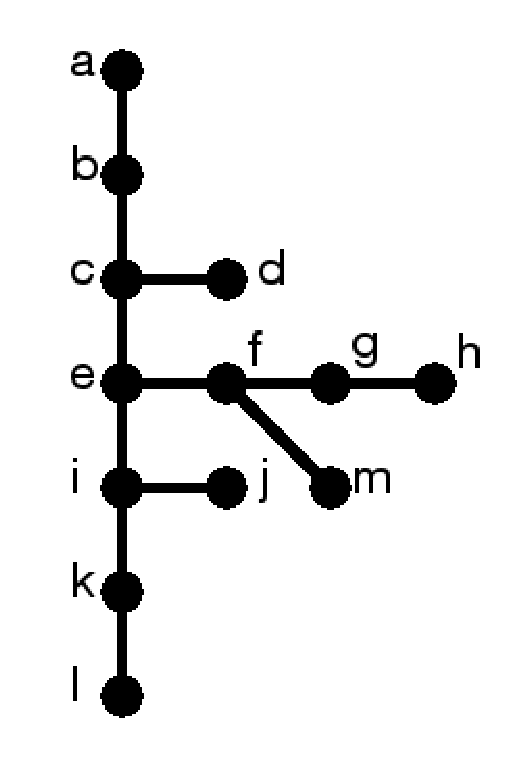
\includegraphics[scale=0.35]{uniqueshortestpathtight}
  \caption{Graph $G$ with $\VC(\range_G)\ge 3$.}
  \label{fig:uniquetight}
\end{figure}

\begin{proof}
%\begin{IEEEproof}
  Consider the graph $G$ in Fig.~\ref{fig:uniquetight}.
  Let $p_1=(a,b,c,e,i,j)$, $p_2=(m,f,e,i,k,l)$, $p_3=(d,c,e,f,g,h)$ be three
  paths. We now show that $Q=\{p_1,p_2,p_3\}$ can be shattered by $\range_G$, which
  implies $\VC(\range_G)\ge 3$. We have $\emptyset=Q\cap\mathcal{T}_a$,
  $\{p_1\}=Q\cap\mathcal{T}_b$,$\{p_2\}=Q\cap\mathcal{T}_k$,
  $\{p_3\}=Q\cap\mathcal{T}_g$, $\{p_1,p_2\}=Q\cap\mathcal{T}_i$,
  $\{p_1,p_3\}=Q\cap\mathcal{T}_c$, $\{p_2,p_3\}=Q\cap\mathcal{T}_f$,
  $\{p_1,p_2,p_3\}=Q\cap\mathcal{T}_e$,  
  Hence all subsets of $Q$ can be expressed as the intersection between $Q$ and
  some range in $\range_G$ which means that $Q$ can be shattered and
  $\VC(\range_G)\ge 3$. Lemma~\ref{lem:vcdimuppboundunique} gives us an upper
  bound $\VC(\range_G)\le3$, so we can conclude that $\VC(\range_G)=3$.
%\end{IEEEproof}
\end{proof}

\section{Algorithm}\label{sec:algo}
In this section we present our algorithm to compute a set of approximations for the
betweenness centrality of all vertices in a graph through sampling, with
probabilistic guarantees on the quality of the approximations.

The intuition behind the algorithm is the following. Given a graph $G=(V,E)$
with vertex-diameter $\Delta_g$ and two parameters $\varepsilon,\delta\in(0,1)$ we first compute a sample
size $k$ using~\eqref{eq:vceapprox} with
$d=\lfloor\log_2(\Delta_G-2)\rfloor+1$:
\begin{equation}\label{eq:samplesize}
k=\frac{c}{\varepsilon^2}\left(\lfloor\log_2(\Delta_G-2)\rfloor+1+\ln\frac{1}{\delta}\right)\enspace.
\end{equation}
The sample size is sufficient to ensure
to achieve the desired accuracy (expressed through $\varepsilon$) with the
desired confidence (expressed through $1-\delta$). Then the algorithm builds a
sample $S$ of $k$ shortest path from $\mathbb{S}_G$ by sampling them according to
the probability distribution $\prob_G$ defined on $\mathbb{S}_G$ as follows:
given a shortest path $p_{uv}\in\mathbb{S}_G$ between a pair of vertices
$(u,v)\in V\times V$, 
\[
\prob_G(p_{uv})=\frac{1}{\binom{n}{2}|\mathcal{S}_{uv}|}\enspace.%=\frac{2}{n(n-1)|\mathcal{S}_{uv}|}\enspace.
\]
Sampling according to $\prob_G$ can be achieved by first picking a pair of distinct vertices $(u,v)$
uniformly at random, computing the set $\mathcal{S}_{uv}$ of all the shortest
paths between $u$ and $v$, and selecting one of these shortest paths uniformly
at random. The estimation $\tilde\betw(v)$ of the betweenness centrality of each
vertex $v\in V$ is obtained by computing the fraction of shortest paths in $S$
that $v$ is internal to and de-normalizing it: 
\[
\tilde\betw(v) = \binom{n}{2}\frac{1}{k}\sum_{p\in S}
\mathds{1}_{\mathsf{Int}(p)}(v) = \binom{n}{2}\frac{1}{k}\sum_{p\in S}
\mathds{1}_{\mathcal{T}_v}(p)\enspace.
\]
Algorithm \ref{alg:algorithm} presents the pseudocode.
\begin{algorithm}[ht]
  \SetKwInOut{Input}{Input}
  \SetKwInOut{Output}{Output}
  \SetKwFunction{VertexDiameter}{getVertexDiameter}
  \SetKwFunction{SamplePair}{sampleVertexPair}
  \SetKwFunction{SampleUniform}{sampleUniformPath}
  \SetKwFunction{PairShortestPaths}{computeAllShortestPaths}
   \DontPrintSemicolon
  %\dontprintsemicolon
  \Input{a graph $G=(V,E)$ with $|V|=n$, real values $\varepsilon,\delta\in(0,1)$}
  \Output{A set of approximations }
  $\Delta_G\leftarrow$\VertexDiameter{G}\label{alg:diamcomp}\; 
  $k\leftarrow (c/\varepsilon^2)(\lfloor\log_2(\Delta_G-2)\rfloor+\ln(1/\delta))$\;
  $S\leftarrow\emptyset$\;
  \For{$i\leftarrow 1$ to $k$} {
  $(u,v)\leftarrow$\SamplePair{$G$}\;
  $\mathcal{S}_{uv}\leftarrow$\PairShortestPaths{$(u,v)$}\;
  $s\leftarrow$\SampleUniform{$\mathcal{S}_{uv}$}\;
  $S\leftarrow S\cup\{s\}$\;
  }
  \For{$v\in V$} {
  $\tilde\betw(v)\leftarrow\binom{n}{2}\sum_{p\in
  S}\mathds{1}_{\mathsf{Int}(p)}(v)$\;
  }
  \Return{$\{\tilde\betw(v), v\in V\}$}
  \caption{Computes approximations $\tilde\betw(v)$ of the betweenness
  centrality $\betw(v)$ for all vertices $v\in V$.}
  \label{alg:algorithm}
\end{algorithm}

The algorithm we describes offers probabilistic guarantees on the quality of all
approximations of the betweenness centrality.
\begin{lemma}\label{lem:correctness}
  With probability at least $1-\delta$, all the approximations computed by the
  algorithm are within $\varepsilon\binom{n}{2}$ from their real value:
  %The algorithm computes a set of approximations $\tilde\betw(v)$ for each $v\in
  %V$ such that
  \[
  \Pr\left(\exists v\in V \mbox{ s.t. }
  |\betw(v)-\tilde\betw(v)|>\varepsilon\binom{n}{2}\right)<\delta\enspace .
  \]
\end{lemma}

\begin{proof}
  Consider the range set $\range_G$ and the probability distribution $\prob_G$.
  For $k$ as in~\eqref{eq:samplesize}, the sample $S$ is a
  $\varepsilon$-approximation to $(\range_G,\prob_G)$ with probability at least
  $1-\delta$. Suppose that this is indeed the case, then from
  Def.~\ref{def:eapprox} and the definition of $\range_G$ we have that
  \[
  \left|\prob_G(\mathcal{T}_v) - \frac{1}{k}\sum_{p\in
  S}\mathds{1}_{\mathcal{T}_v}(p)\right|=\left|\prob_G(\mathcal{T}_v) -
  \frac{1}{\binom{n}{2}}\tilde\betw(v)\right|\le\varepsilon, \forall v\in
  V\enspace.
  \]
  From the definition of $\prob_G$ we have
  \[
  \prob_G(\mathcal{T}_v)=\frac{1}{\binom{n}{2}}\sum_{p_{uw}\in\mathcal{T}_v}\frac{1}{|\mathcal{S}_{uw}|}=\frac{1}{\binom{n}{2}}\betw(v),
  \]
  which concludes the proof.
\end{proof}

\paragraph{Unique shortest paths case.} When the graph $G$ is undirected and
there is an unique shortest path between each pair of node, then one can apply
Lemma~\ref{lem:vcdimuppboundunique} and obtain a smaller sample size
\[ k= \frac{c}{\varepsilon^2}\left(2+\ln\frac{1}{\delta}\right)
\]
to approximate the betweenness centralities of all the vertices. Unique shortest
paths are common in or even enforced in road networks~\citep{GeisbergerSS08} by
slightly perturbing the edge weights or having a deterministic tie breaking
policy.

\subsection{Approximating the diameter}\label{sec:diam}
The algorithm presented in the previous section requires the knowledge (or the
computation) of the vertex-diameter $\Delta_G$) of the graph $G$ (line
\ref{alg:diamcomp} of Alg.~\ref{alg:algorithm}). Computing $\Delta_G$ exactly
can be done by finding the shortest paths between all pair of vertices in $V$
and computing the maximum size. This can be done in time \XXX. Such an exact
computation would defeat our purposes, because once we have all the shortest
paths, we can compute the betweenness of all the nodes exactly. Given that
Thm.~\ref{thm:eapprox} only requires an upper bound to the VC-dimension of the
range set, an upper bound to the vertex-diameter would be sufficient for our
purposes, provided its computation is fast and it does not result in a much
larger sample size than if we used the exact value for $\Delta_G$. There are
known algorithms to approximate the diameter of a
graph~\citep{AingwordCIM99,BoitmanisFL06,RodittyW12}, with various running times
and quality of approximations.

For our case, if $G$ is \emph{undirected} and \emph{all the weights are
unitary}, a $2$-approximation to $\Delta_G$ is sufficient and can be computed in
time \XXX by selecting a vertex $v\in V$ uniformly at random, computing the
shortest paths from $v$ to all other vertices in $V$, and taking
$\tilde\Delta_G$ to be the sum of the sizes of the two longest shortest paths
from $v$ to two distinct other nodes $u$ and $w$. 

\begin{lemma}\label{lem:diam}
  $\Delta_G\le\tilde\Delta_G\le 2\Delta_G$.
\end{lemma}
\begin{proof}
  Let $p_{vu}$ be the shortest path between $v$ and $u$ and analogously
  $p_{vw}$. We have $\tilde\Delta_G\le 2\Delta_G$ because
  $|p_{vu}|,|p_{vw}|\le\Delta_G$, so $|p_{vu}|+|p_{vw}|\le 2\Delta_g$. To see
  that $\tilde\Delta_G\ge\Delta_G$, consider a pair of nodes $x$ and $z$ such
  that the size of a shortest path between $x$ and $z$ is equal to $\Delta_G$.
  Let $p_{xv}$ be a shortest path between $x$ and $v$ and let $p_{vz}$ be a
  shortest path between $v$ and $z$. 
  Then (by the triangle inequality? \XXX)
  \[
  |p_{xv}|+|p_{vz}|=|p_{vx}|+|p_{vz}|\ge\Delta_G\enspace.
  \]
  It is easy to see that $|p_{vu}|+|p_{vw}|\ge|p_{vx}|+|p_{vz}|$ because the
  vertices $u$ and $w$ are chosen so that to maximize this sum. Hence
  \[
  \tilde\Delta_G = |p_{vu}|+|p_{vw}| \ge\Delta_G\enspace.\qedhere
  \]
\end{proof}

The impact of using $\tilde\Delta_G$ when computing the sample size $k$ is that
the sample will contain at most $c/\varepsilon^2$ more paths than if we used the
exact value $\Delta_G$. The computation of $\tilde\Delta_G$ has no (\XXX or
minimal) impact on the running time of our algorithm: once the $\Delta_G$ has
been computed, we can sample another node $u\neq v$ and then sample one of the
(already computed) shortest paths between $v$ and $v$ and use this path as first
element of the sample.

\subsection{Discussion}
\XXX TBD: running time, worst case, comparison with best previous work.

\citet{BrandesP07} present an algorithm that also uses sampling to approximate
the betweenness centrality of all the vertices of the graph. The algorithm
create a sample $S=\{v_1,\dotsc,v_k\}$ of $k$ vertices drawn uniformly at random 
and computes all the shortest paths between each $v_i$ to all other vertices in
the graph. The estimation $\tilde\betw'(u)$ for the betweenness centrality
$\betw(u)$ is
\[ 
\tilde\betw'(u)= \frac{n}{k}\sum_{v_i\in S}\sum_{w\neq v_i,w\neq
u}\sum_{p\in\mathcal{S}_{v_iw}}\frac{\mathds{1}_{\mathsf{Int}(p)}(u)}{|\mathcal{S}_{v_iw}|},
\]
As it was for our algorithm, the key ingredient to ensure a correct
approximation for the betweenness centrality is the computation of the sample
size $k$. Inspired by the work of~\citet{EppsteinW04}, \citet{BrandesP07} rely
on the following classical result by~\citet{Hoeffding63} for their computation
of $k$.

\begin{theorem}[\citep{Hoeffding63}]
  Let $X_1,X_2,\dotsc,X_k$ be a sequence of independent random variables
  such that $a_i\leq X_i\leq b_i$. Then for any $\xi > 0$
  \begin{equation}\label{eq:hoeffding}
    \Pr\left(\frac{|X_1+\dotsb+X_k|}{k}-\mathbf{E}\left[\frac{|X_1+\dotsb+X_k|}{k}\right]|\geq
    \xi\right)\leq 2e^{-2k^2\xi^2/\sum_{i=1}^{k}(b_{i}-a_{i})^2}\enspace.
  \end{equation}
\end{theorem}

\citet{BrandesP07} use this result to compute a sample size $k$ sufficient to ensure that, for
a fixed vertex $u$,
\[ 
\Pr\left(|\betw(u)-\tilde\betw'(u)|>\varepsilon\binom{n}{2}\right)<\frac{\delta}{n}\enspace.
\]
In their setting $\xi=\varepsilon\binom{n}{2}$ and there is a variable $X_i$ for
each vertex $v_i$ in the sample:
\[ 
X_i=n\sum_{w\neq v_i,w\neq
u}\sum_{p\in\mathcal{S}_{v_iw}}\frac{\mathds{1}_{\mathsf{Int}(p)}(u)}{|\mathcal{S}_{v_iw}|}\enspace
.
\]
It is easy to see that $0\le X_i\le n(n-2)$. Moreover,
\begin{align*}
\mathbf{E}\left[\frac{|X_1+\dotsb+X_k|}{k}\right] &=
\frac{n}{k}\mathbf{E}\left[\sum_{v_i\in S}\sum_{w\neq v_i,w\neq
u}\sum_{p\in\mathcal{S}_{v_iw}}\frac{\mathds{1}_{\mathsf{Int}(p)}(u)}{|\mathcal{S}_{v_iw}|}\right]
=\frac{n}{k}\sum_{v\in V}\mathbf{E}\left[Y_v\sum_{w\neq v,w\neq
u}\sum_{p\in\mathcal{S}_{vw}}\frac{\mathds{1}_{\mathsf{Int}(p)}(u)}{|\mathcal{S}_{vw}|}\right] =
\\
&=\frac{n}{k}\sum_{v\in V}\mathbf{E}[Y_v]\sum_{w\neq v,w\neq
u}\sum_{p\in\mathcal{S}_{vw}}\frac{\mathds{1}_{\mathsf{Int}(p)}(u)}{|\mathcal{S}_{vw}|}
=\frac{n}{k}\sum_{v\in V}\frac{k}{n}\sum_{w\neq v,w\neq
u}\sum_{p\in\mathcal{S}_{vw}}\frac{\mathds{1}_{\mathsf{Int}(p)}(u)}{|\mathcal{S}_{vw}|}
= \betw(u),
\end{align*}
where $Y_v$ is a Bernoulli random variable taking value 1 if $v\in S$, and 0
otherwise, so $\Pr(Y_v=1)=k/n$.

Plugging these values in~\eqref{eq:hoeffding}, we have
\[
\Pr\left(|\betw(u)-\tilde\betw'(u)|>\varepsilon\binom{n}{2}\right)\leq
2e^{-2k^2\varepsilon^2\left(\frac{n(n-1)}{2}\right)^2/kn^2(n-2)^2}=2e^{-k\epsilon^2(n-1)^2/2(n-2)^2}\enspace.
\]
We want this probability to be at most $\delta/n$, so we need a sample of size
\[
k\geq \frac{2(n-2)^2}{\varepsilon^2(n-1)^2}\left(\ln n
+\ln\frac{1}{\delta} +\ln 2\right)\enspace.
\]
An application of the union bound over the $n$ vertices ensures a uniform guarantee on the quality of
all the estimation, with probability at least $1-\delta$.


\begin{figure}
  \centering
  \begin{subtable}{\textwidth}
	\centering
	\ifdmkd
	  \caption{Undirected graphs}
	  \label{tab:expUndir}
	\fi
  \begin{small}
    \begin{tabular}{cccccc}
      \toprule
      &  & & &  \multicolumn{2}{c}{$\frac{\mbox{Time}_\mathsf{BP}}{\mbox{Time}_\mathsf{VC}}$} \\
      \cmidrule(r){5-6}
      & \multicolumn{3}{c}{Graph Properties} & \multicolumn{2}{c}{diam-2approx} \\
      \cmidrule(r){2-4} \cmidrule(r){5-6}
      Graph & $|V|$ & $|E|$ & $\VD(G)$ & min & max \\
      \midrule
      oregon1-010331 & 10,670 & 22,002 & 9 & 4.39 & 4.75\\  % [1ex] adds vertical space
      oregon1-010526 & 11,174 & 23,409 & 10 & 4.26 & 4.73 \\
      ca-HepPh & 12,008 & 237,010 & 13 & 3.06 & 3.33\\
      ca-AstroPh & 18,772 & 396,160  & 14 & 3.26 & 3.76\\
      ca-CondMat & 23,133 & 186,936 & 15 & 3.75 & 4.08\\
      email-Enron & 36,692 & 421,578 & 12 & 3.60 & 4.16\\
      \bottomrule
    \end{tabular}
  \end{small}
  \ifdmkd
  \else
  \caption{Undirected graphs}
  \label{tab:expUndir}
  \fi
  \end{subtable}
\ifproof
\\
\else
\hspace{-5pt}
\fi
  \begin{subtable}{\textwidth}
	\centering
	\ifdmkd
	\caption{Directed graphs}
	\label{tab:expDir}
	\fi
  \begin{small}
    \begin{tabular}{cccccccc}
      \toprule
      & & & & \multicolumn{4}{c}{$\frac{\mbox{Time}_\mathsf{BP}}{\mbox{Time}_\mathsf{VC}}$} \\
      \cmidrule(r){5-8}
      & \multicolumn{3}{c}{Graph Properties} & \multicolumn{2}{c}{diam-exact} &
      \multicolumn{2}{c}{diam-UB} \\
      \cmidrule(r){2-4} \cmidrule(r){5-6} \cmidrule(r){7-8}
      Graph & $|V|$ & $|E|$ & $\VD(G)$ & min & max & min & max \\
      \midrule
      wiki-Vote & 7,115 & 103,689  & 7 & 3.35 & 3.69 & 1.05 & 1.27 \\
      p2p-Gnutella25 & 22,687 & 54,705 & 11 & 5.45 & 5.78 & 1.94 & 2.09 \\
      cit-HepTh & 27,770 & 352,807 & 14 & 3.58 & 3.83 & 1.39 & 1.61 \\
      cit-HepPh & 34,546 & 421,578 & 12 & 4.91 & 5.01 & 1.60 & 1.71 \\ 
      p2p-Gnutella30 & 36,682 & 88,328 & 10 & 5.02 & 5.46 & 2.08 & 2.22\\
      soc-Epinions1 & 75,879 & 508,837 & 13 & 4.20 & 4.25 & 1.35 & 1.38\\
      \bottomrule
    \end{tabular} 
  \end{small}
  \ifdmkd
  \else
  \caption{Directed graphs}
  \label{tab:expDir}
  \fi
  \end{subtable}
  \caption{Graph characteristics and running time ratios.}
  \label{fig:tables}
\end{figure}

\section{Experimental evaluation}\label{sec:exper}
We conducted an experimental evaluation of our algorithms, with two major
driving goals in mind: study the behavior of the algorithms presented in this
paper and compare it with that of other related
algorithms~\citep{Brandes01,BrandesP07,JacobKLPT05,GeisbergerSS08}, in terms of
accuracy of the estimation, execution time, work performed, and scalability as
function of the network size.
\ifproof 
\else
Due to space limitations, we only report a subset
of our results and refer the reader to the extended online version of the
paper~\citep{RiondatoK13}.
\fi

\paragraph{Implementation and environment}
We implemented our algorithms\footnote{The implementations are available at
\url{http://cs.brown.edu/~matteo/centrsampl.tar.bz2}. An independent
implementation of our algorithms is available in NetworKit~\citep{StaudtSM14}.},
the one presented by~\citet{BrandesP07} and~\citet{JacobKLPT05} and the linear scaling
version by~\citet{GeisbergerSS08} in C, by extending the implementation of the
exact algorithm~\citep{Brandes01} contained in igraph~\citep{igraph}.
The implementations are similarly engineered, given that they are based on the
same subroutines for the computation of the shortest path (Dijkstra's algorithm
for weighted graphs, BFS for unweighted ones), and they received similar amounts
of optimization. We exposed our implementations through Python 3.3.1, which was
used for running the simulations. We run the experiments on a quad-core AMD
Phenom\texttrademark II X4 955 Processor with 16GB of RAM, running Debian
\emph{wheezy} with a Linux kernel version 3.2.0.

\paragraph{Datasets} In our evaluation we used a number of graphs from the
Stanford Large Network Dataset
Collection\footnote{\url{http://snap.stanford.edu/data/index.html}}. These are
all real world datasets including online social networks, communication (email)
networks, scientific citation and academic collaboration networks, road
networks, Amazon frequent co-purchased product networks, and more. Basic
information about the graphs we used are reported in the two leftmost columns 
of Figs.~\ref{tab:expDir} and~\ref{tab:expUndir}. We refer the
reader to the SLNDC website for additional details about each dataset. 
To evaluate scalability we also created a number of artificial graphs of
different sizes (1,000 to 100,000 vertices) using the Barab\'asi-Albert
model~\citep{BarabasiA99} as implemented by igraph~\citep{igraph}. 
%\XXX Are there parameters of the Barabasi-Albert model we should mention?

\paragraph{Diameter approximation}
As we discussed in the previous sections the number of samples that the proposed
algorithm requires depends on the vertex-diameter of the graph. 
For the computation of the vertex-diameter in case of undirected graphs we used
the 2-approximation algorithm that we briefly described in Sect.~\ref{sec:algo}.
We denote this as ``diam-2-approx'' when reporting results in this section. For
directed graphs, we computed the number of samples using both the exact value of
the vertex-diameter (indicated as diam-exact) as well as the trivial upper bound
$|V|-2$ (indicated as diam-UB). 


%\begin{table*}[ht]
%  \centering   
%  \begin{small}
%    \begin{tabular}{cccccc}
%      \toprule
%      & \multicolumn{3}{c}{Graph Properties} & \multicolumn{2}{c}{$\frac{\mbox{Time}_\mathsf{BP}}{\mbox{Time}_\mathsf{VC}}$} \\
%      \cmidrule(r){2-4} \cmidrule(r){5-6}
%      Graph & $|V|$ & $|E|$ & $\VD(G)$ & min & max \\
%      \midrule
%      oregon1-010331 & 10,670 & 22,002 & 9 & 4.39 & 4.75\\  % [1ex] adds vertical space
%      oregon1-010526 & 11,174 & 23,409 & 10 & 4.26 & 4.73 \\
%      ca-HepPh & 12,008 & 237,010 & 13 & 3.06 & 3.33\\
%      ca-AstroPh & 18,772 & 396,160  & 14 & 3.26 & 3.76\\
%      ca-CondMat & 23,133 & 186,936 & 15 & 3.75 & 4.08\\
%      email-Enron & 36,692 & 421,578 & 12 & 3.60 & 4.16\\[1ex] % inserting body of the table
%      \bottomrule
%    \end{tabular}
%  \end{small}
%  \caption{Graph properties for undirected graphs and ratios between running times
%for $\varepsilon=$\XXX and $\delta=0.1$.}
%  \label{tab:expUndir}
%\end{table*}

%  \begin{small}
%\begin{tabular}{|c c c c |c c |c  c |} % centered columns (5 columns)
%\hline\hline %inserts double horizontal lines
%Graph & Node & Edges & Diameter  & \multicolumn{2}{|c|}{$\frac{\varepsilon\mbox{-Edges-BP}}{ \varepsilon\mbox{-Edges-VC}}$} & \multicolumn{2}{c|}{$\frac{\varepsilon\mbox{-Time-BP}}{\varepsilon\mbox{-Time-VC}}$}\\ [0.5ex] % inserts table 
%\hline
%&  &  & &\multicolumn{4}{|c|}{diam-2-approx} \\
%\hline
%&  &  & & min & max & min & max\\
%%heading
%\hline % inserts single horizontal line
%%\multirow{6}{35mm}{\begin{sideways}\parbox{15mm}{Undirected\\ diam-approx}\end{sideways}}\\
%oregon1-010331 & 10,670 & 22,002 & 9 & 3.69 & 3.73 & 4.39 & 4.75\\  % [1ex] adds vertical space
%oregon1-010526 & 11,174 & 23,409 & 10 &  3.53 & 3.74 & 4.26 & 4.73 \\
%ca-HepPh & 12,008 & 237,010 & 13  & 2.43 & 2.49 & 3.06 & 3.33\\
%ca-AstroPh & 18,772 & 396,160  & 14  & 2.81 & 2.95 & 3.26 & 3.76\\
%ca-CondMat & 23,133 & 186,936 & 15  & 3.24 & 3.26 & 3.75 & 4.08\\
%email-Enron & 36,692 & 421,578 & 12  & 2.98 & 3.18 & 3.60 & 4.16\\[1ex] % inserting body of the table
%\hline %inserts single line


%\begin{table*}[ht]
%  \centering
%  \begin{small}
%    \begin{tabular}{cccccccc}
%      \toprule
%      & & & & \multicolumn{4}{c}{$\frac{\mbox{Time}_\mathsf{BP}}{\mbox{Time}_\mathsf{VC}}$} \\
%      \cmidrule(r){5-8}
%      & \multicolumn{3}{c}{Graph Properties} & \multicolumn{2}{c}{diam-exact} &
%      \multicolumn{2}{c}{diam-UB} \\
%      \cmidrule(r){2-4} \cmidrule(r){5-6} \cmidrule(r){7-8}
%      Graph & $|V|$ & $|E|$ & $\VD(G)$ & min & max & min & max \\
%      \midrule
%      wiki-Vote & 7,115 & 103,689  & 7 & 3.35 & 3.69 & 1.05 & 1.27 \\
%      p2p-Gnutella25 & 22,687 & 54,705 & 11 & 5.45 & 5.78 & 1.94 & 2.09 \\
%      cit-HepTh & 27,770 & 352,807 & 14 & 3.58 & 3.83 & 1.39 & 1.61 \\
%      cit-HepPh & 34,546 & 421,578 & 12 & 4.91 & 5.01 & 1.60 & 1.71 \\ 
%      p2p-Gnutella30 & 36,682 & 88,328 & 10 & 5.02 & 5.46 & 2.08 & 2.22\\
%      soc-Epinions1 & 75,879 & 508,837 & 13 & 4.20 & 4.25 & 1.35 & 1.38\\ 
%      \bottomrule
%    \end{tabular} 
%  \end{small}
%  \caption{\XXX}
%  \label{tab:expDir} % is used to refer this table in the text
%\end{table*}

%\begin{tabular}{|c c c c | c c | c c | c c | c c | c c | c c|} % centered columns (5 columns)
%\hline\hline %inserts double horizontal lines
%Graph & Node & Edges & Diameter  & \multicolumn{2}{|c|}{$\frac{\varepsilon\mbox{-Edges-BP}}{ \varepsilon\mbox{-Edges-VC}}$} & \multicolumn{2}{c|}{$\frac{\varepsilon\mbox{-Time-BP}}{\varepsilon\mbox{-Time-VC}}$} & \multicolumn{2}{c|}{$\frac{\varepsilon\mbox{-Edges-BP}}{ \varepsilon\mbox{-Edges-VC}}$} & \multicolumn{2}{c|}{$\frac{\varepsilon\mbox{-Time-BP}}{\varepsilon\mbox{-Time-VC}}$} & \multicolumn{2}{c|}{$\frac{\varepsilon\mbox{-Edges-BP}}{ \varepsilon\mbox{-Edges-VC}}$} & \multicolumn{2}{c|}{$\frac{\varepsilon\mbox{-Time-BP}}{\varepsilon\mbox{-Time-VC}}$}\\ [0.5ex] % inserts table 
%\hline
%&  &  & &\multicolumn{4}{|c|}{diam-exact}  &  \multicolumn{4}{c|}{diam-UB} & \multicolumn{4}{c|}{Top-K}\\
%%heading
%\hline % inserts single horizontal line
%&  &  & &min & max & min & max&min & max & min & max &min & max & min & max\\
%\hline % inserts single horizontal line
%%\multirow{6}{13mm}{\begin{sideways}\parbox{15mm}{Directed}\end{sideways}}\\
%wiki-Vote & 7,115 & 103,689  & 7 & 2.99 & 3.10 & 3.35 & 3.69 & 1.04 & 1.06 &1.05 & 1.27 & - & - & - & -\\
%p2p-Gnutella25 & 22,687 & 54,705 & 11 & 5.02 & 5.46 & 5.45 & 5.78 & 1.85& 1.94& 1.94 & 2.09 & - & - & - &-\\
%cit-HepTh & 27,770 & 352,807 & 14  & 2.71 & 2.86 & 3.58 & 3.83 & 1.17 & 1.21 & 1.39 & 1.61 & - & -  & - & -\\
%cit-HepPh & 34,546 & 421,578 & 12 & 3.51 & 3.68 & 4.91 & 5.01 & 1.20 & 1.25& 1.60 & 1.71 & - & -  &-  &-\\ % inserting body of the table
%p2p-Gnutella30 & 36,682 & 88,328 & 10  & 5.33 & 5.63 & 5.02 & 5.46 & 1.92 & 1.99 & 2.08 & 2.22 & - & - & - & -\\
%soc-Epinions1 & 75,879 & 508,837 & 13  & 3.06&  3.11 & 4.20 & 4.25 & 1.00 & 1.03 & 1.35 & 1.38 & - &  - & - & -\\ [1ex] % [1ex] adds vertical space
%\hline %inserts single line
%\end{tabular}
%\end{small}
%\caption{\XXX
%%For each graph efficiency measures generated  for a given input  as the average of 5 runs for a  pair of given values $\varepsilon,\delta$.
%%The value of $\delta$ was 0.1 and $\varepsilon$ took values 0.01, 0.015, 0.02, 0.04, 0.06, 0.08, 0.1.
%%Among the 6 data points that produced with varied $\varepsilon$ we present the minimum and maximum ratios of the Brandeis-Pitch method over VC-dimension method for the number of touched edges during the execution and time.
%%In both undirected and directed graphs the exact value of the diameter was used. For each ($\varepsilon,\delta$) the experiment was repeated 5 times and the average was recorded.
%}
%\label{tab:expDir} % is used to refer this table in the text
%\end{table*}
\begin{figure*}[htbp]
  \centering
  \begin{subfigure}[b]{1\textwidth}
  \centering
    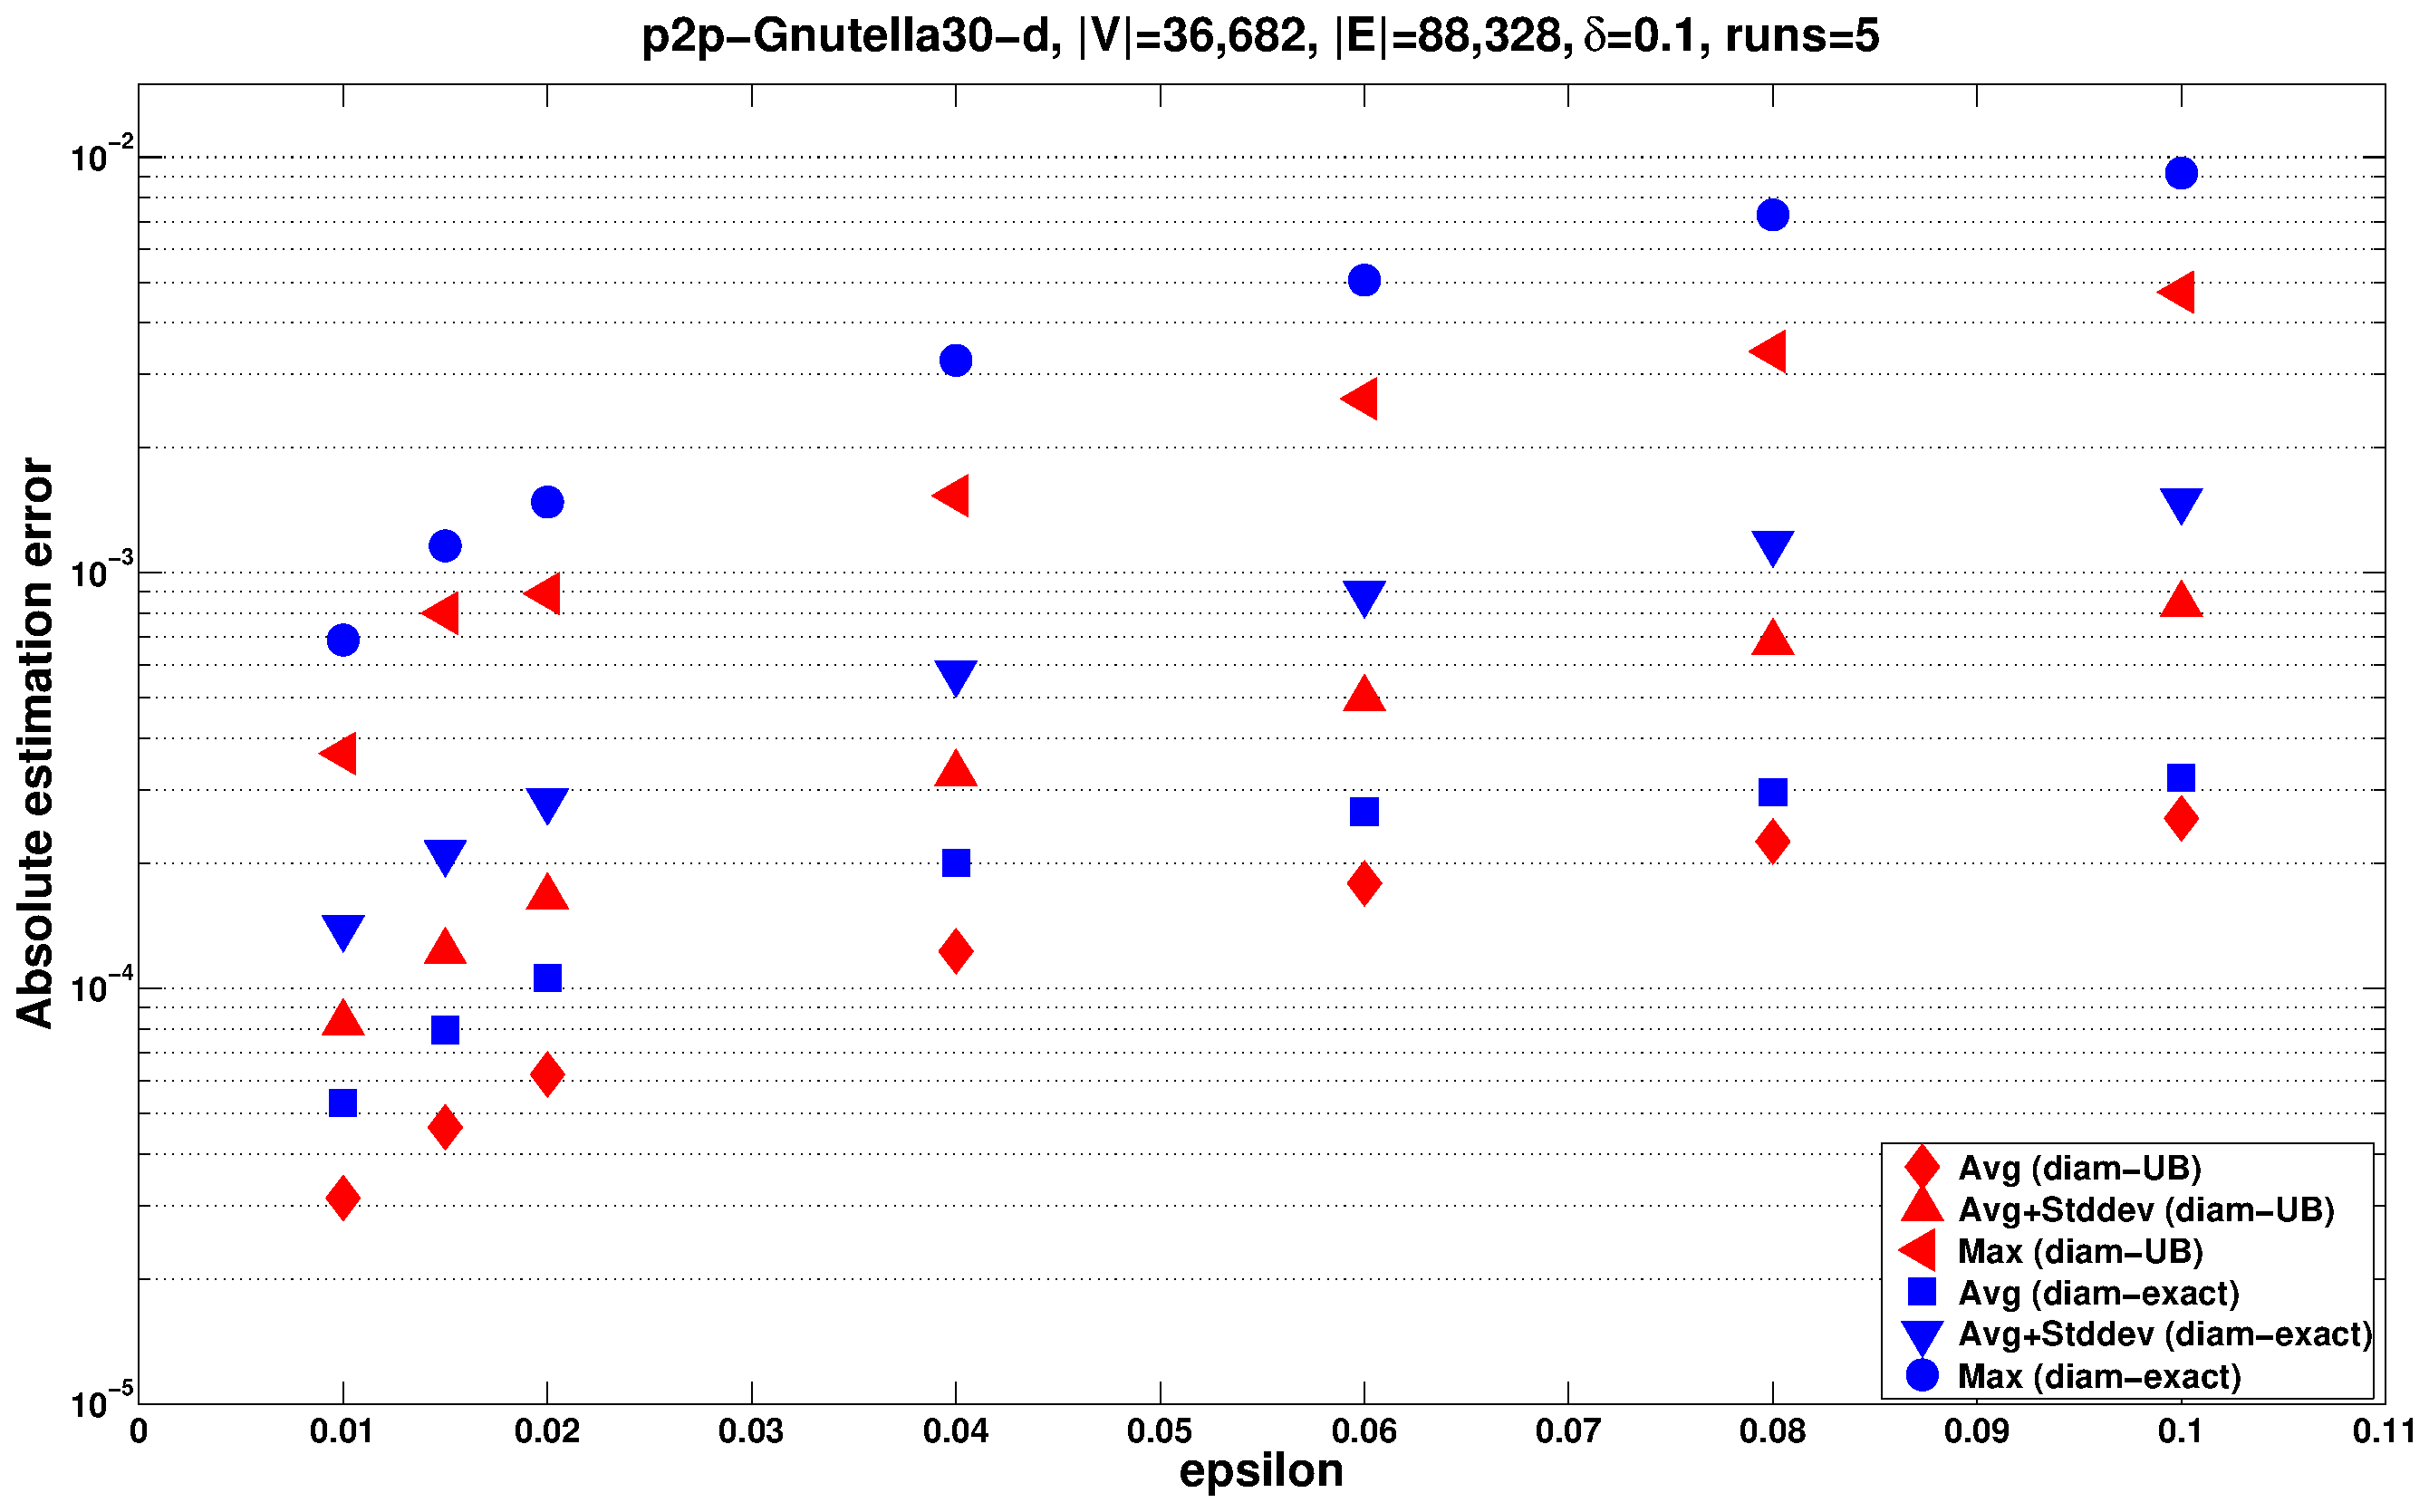
\includegraphics[width=\textwidth,height=0.18\textheight]{figures/eps/p2p-Gnutella30-error}
    \caption{p2p-Gnutella30 (directed)}
    \label{fig:gnutella:error}
  \end{subfigure}
  %\ifproof
  %\hfill

  \begin{subfigure}[b]{1\textwidth}
	\centering
    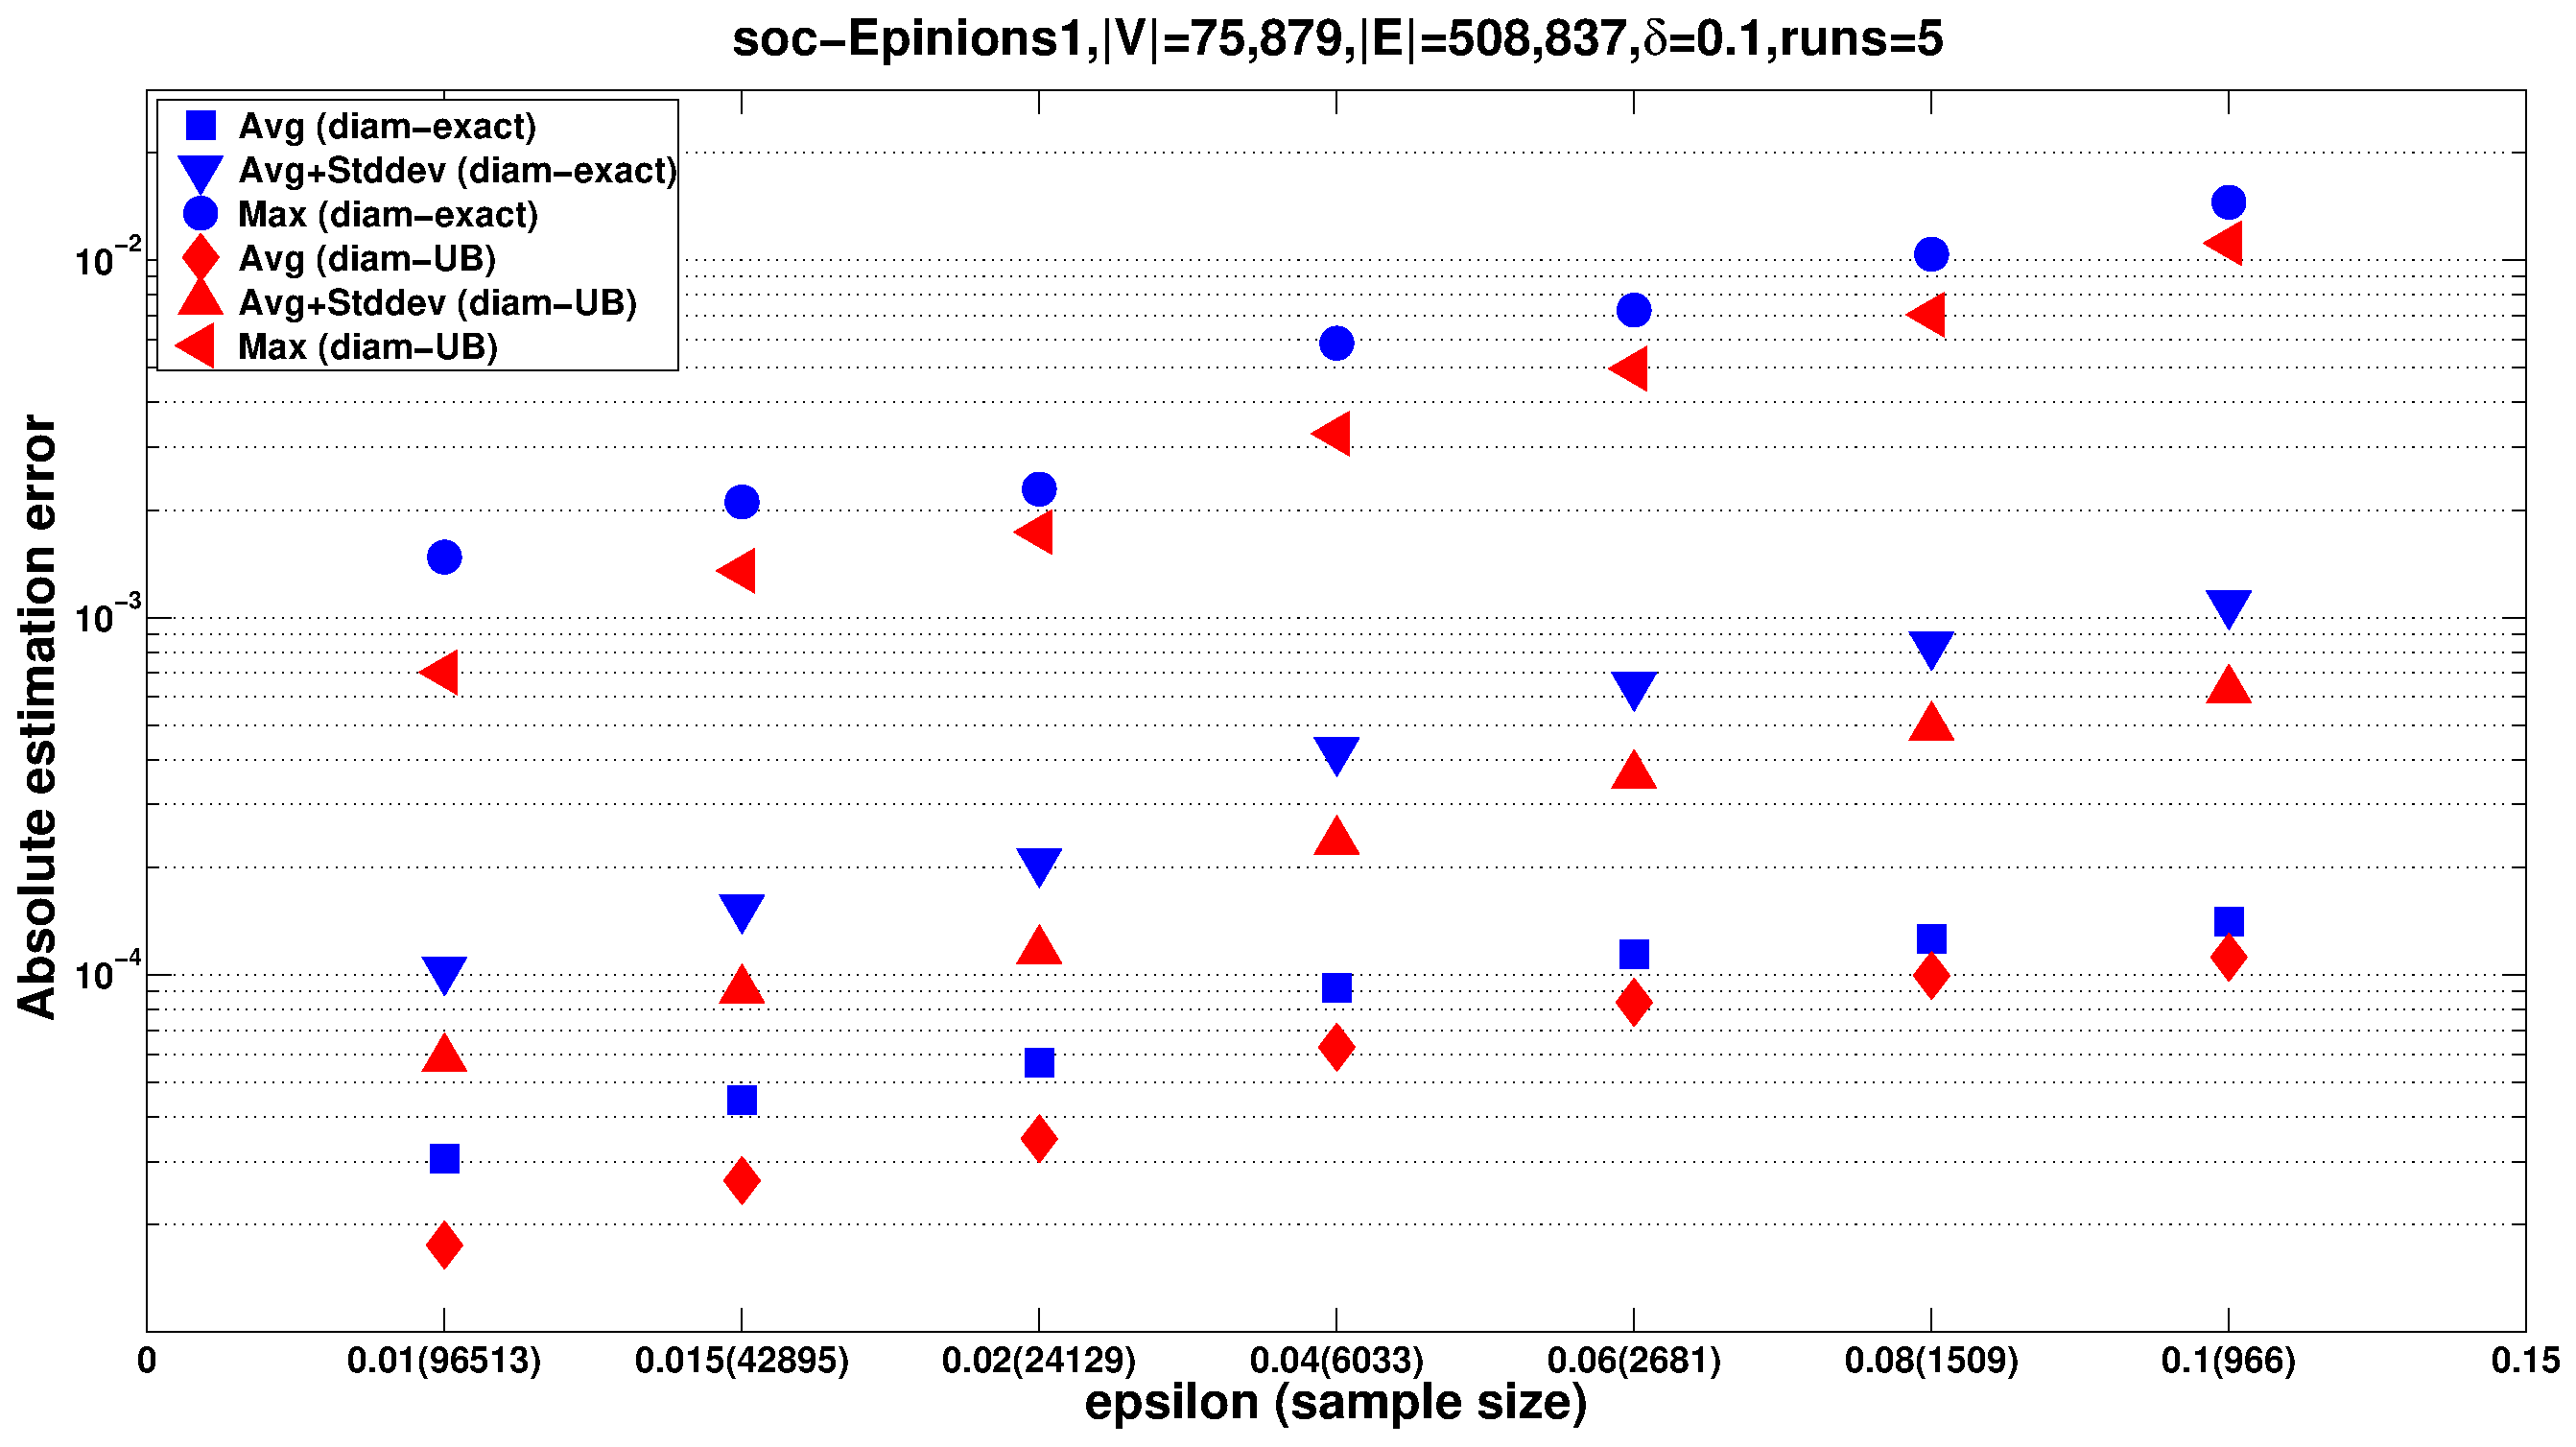
\includegraphics[width=\textwidth,height=0.18\textheight]{figures/eps/soc-Epinions1-error}
    \caption{soc-Epinions1 (directed)}
    \label{fig:Epinions:error}
  \end{subfigure}

  \begin{subfigure}[b]{1\textwidth}
	\centering
    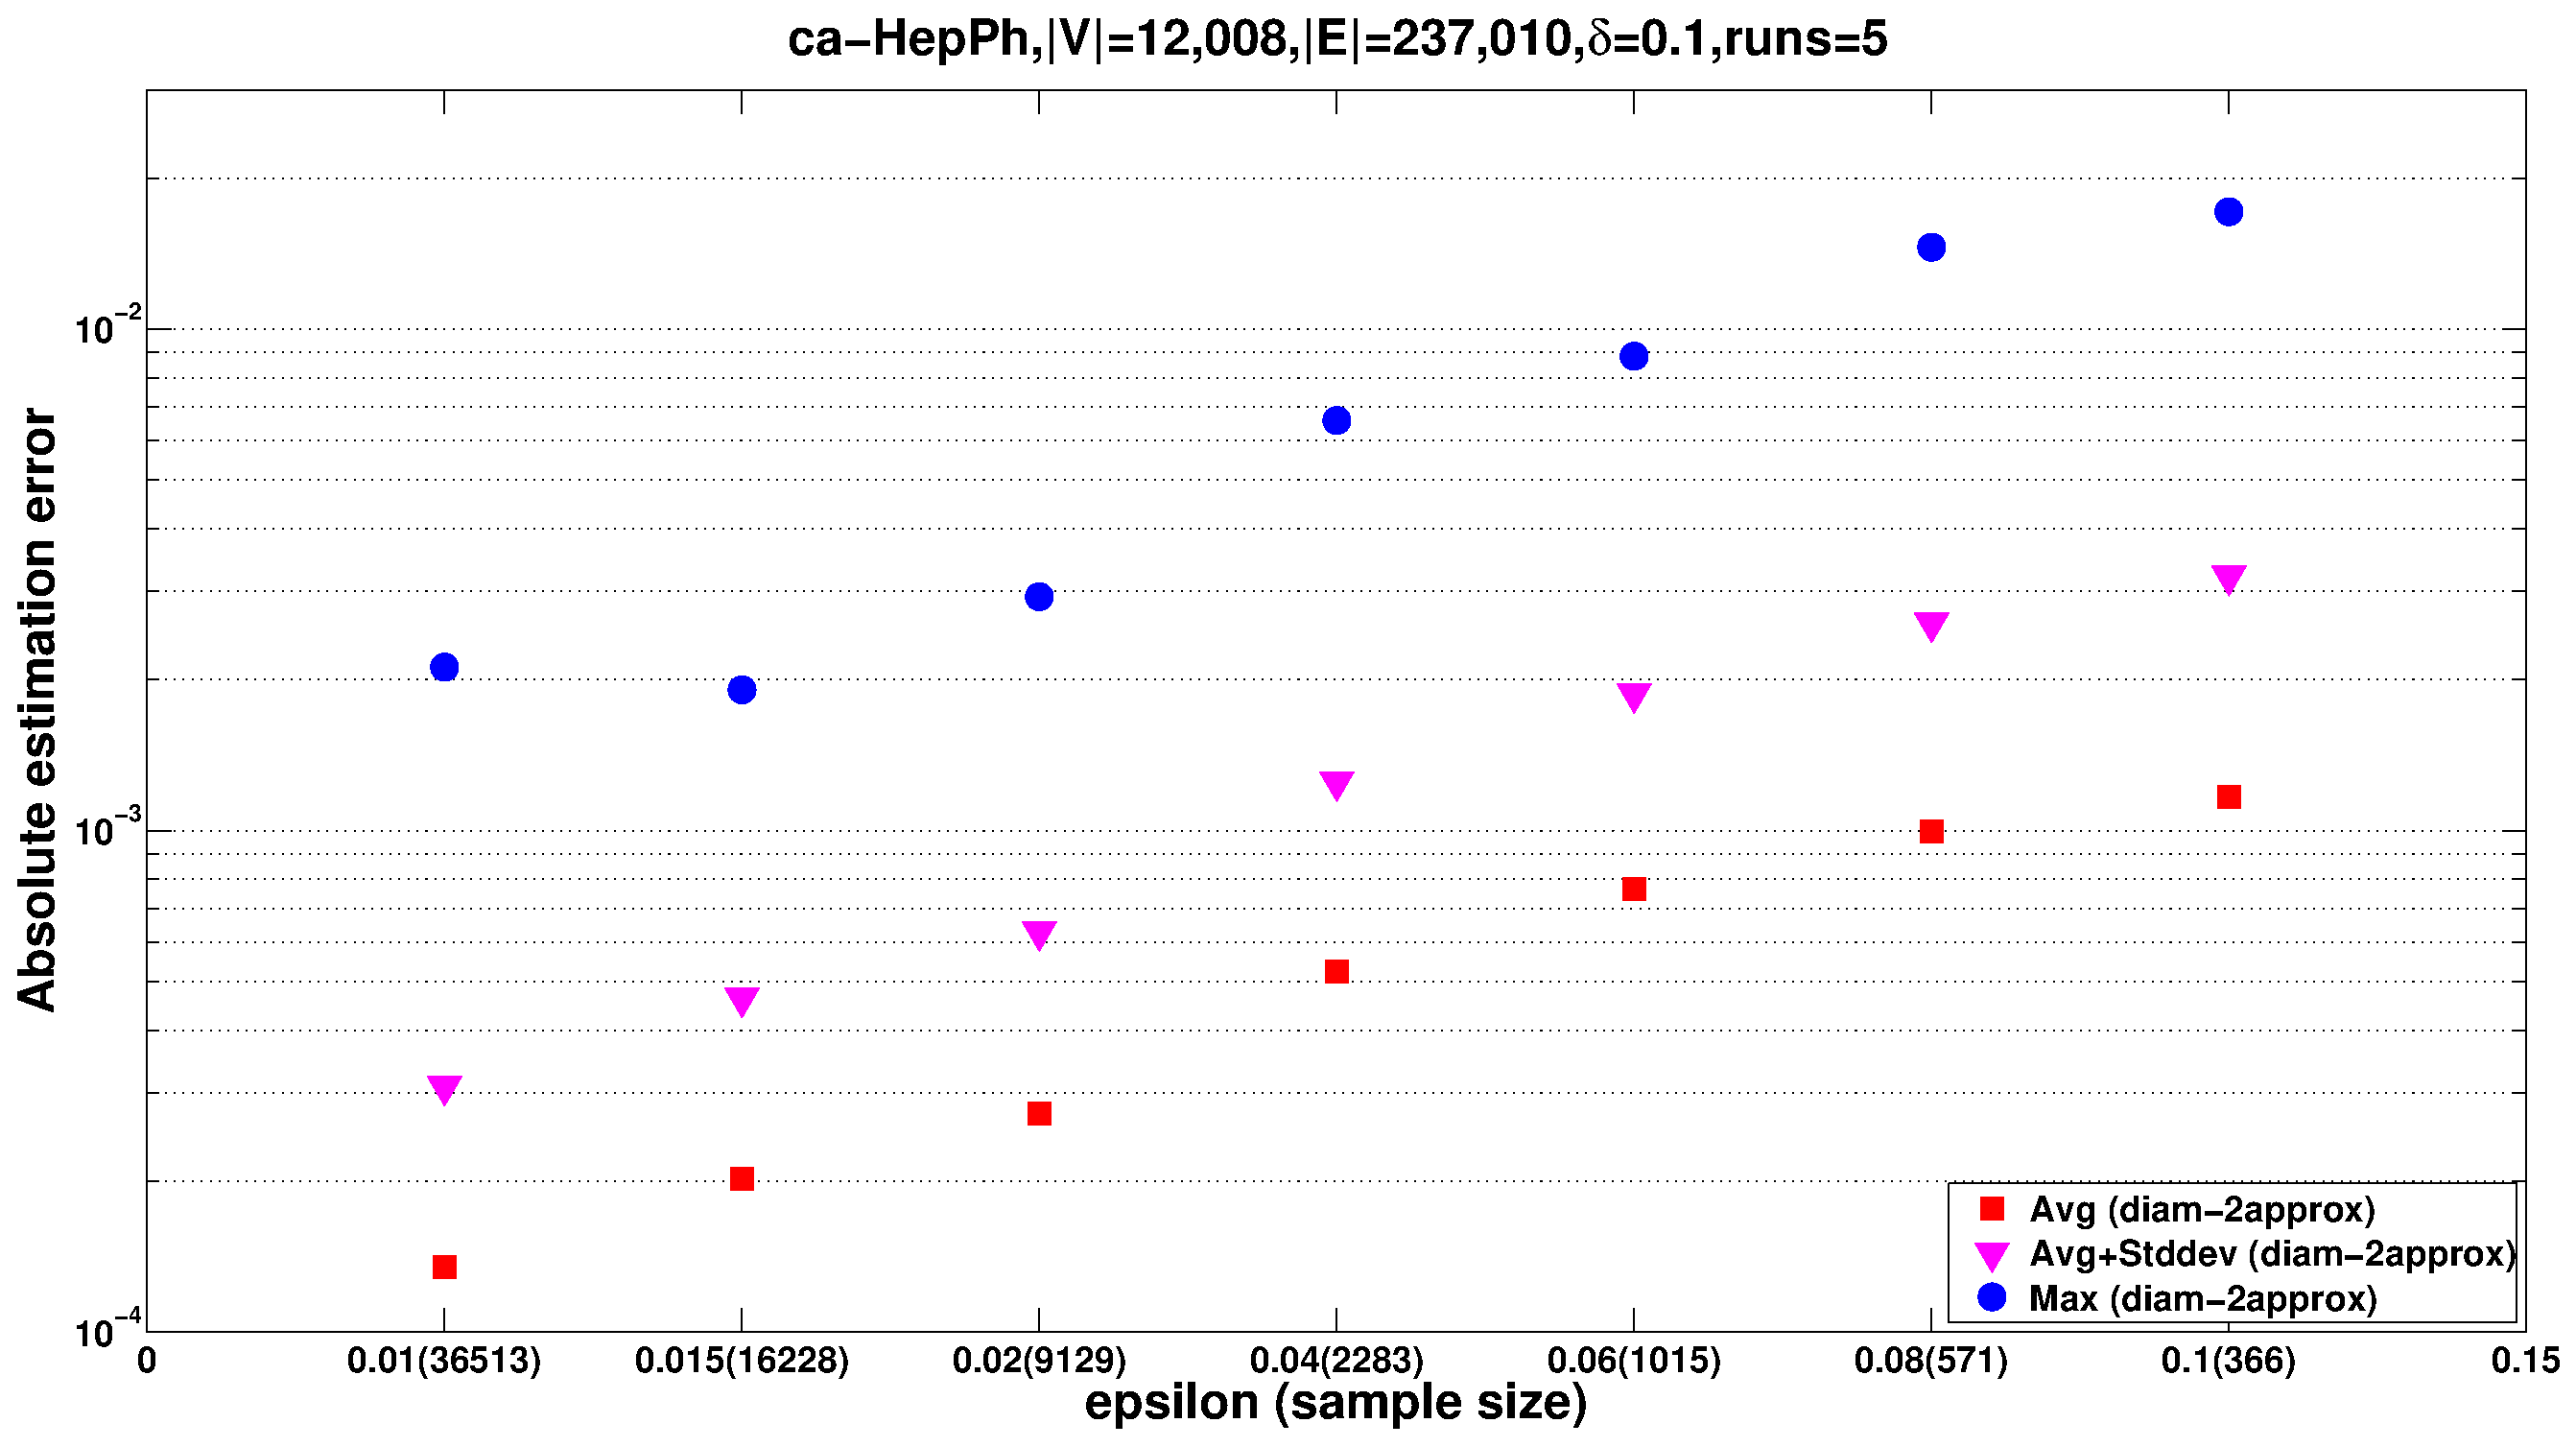
\includegraphics[width=\textwidth,height=0.18\textheight]{figures/eps/ca-HepPh-error}
    \caption{ca-HepPh (undirected)}
    \label{fig:HepPh:error}
  \end{subfigure}
  %\fi
  %\hfill

  \begin{subfigure}[b]{1\textwidth}
  \centering
    %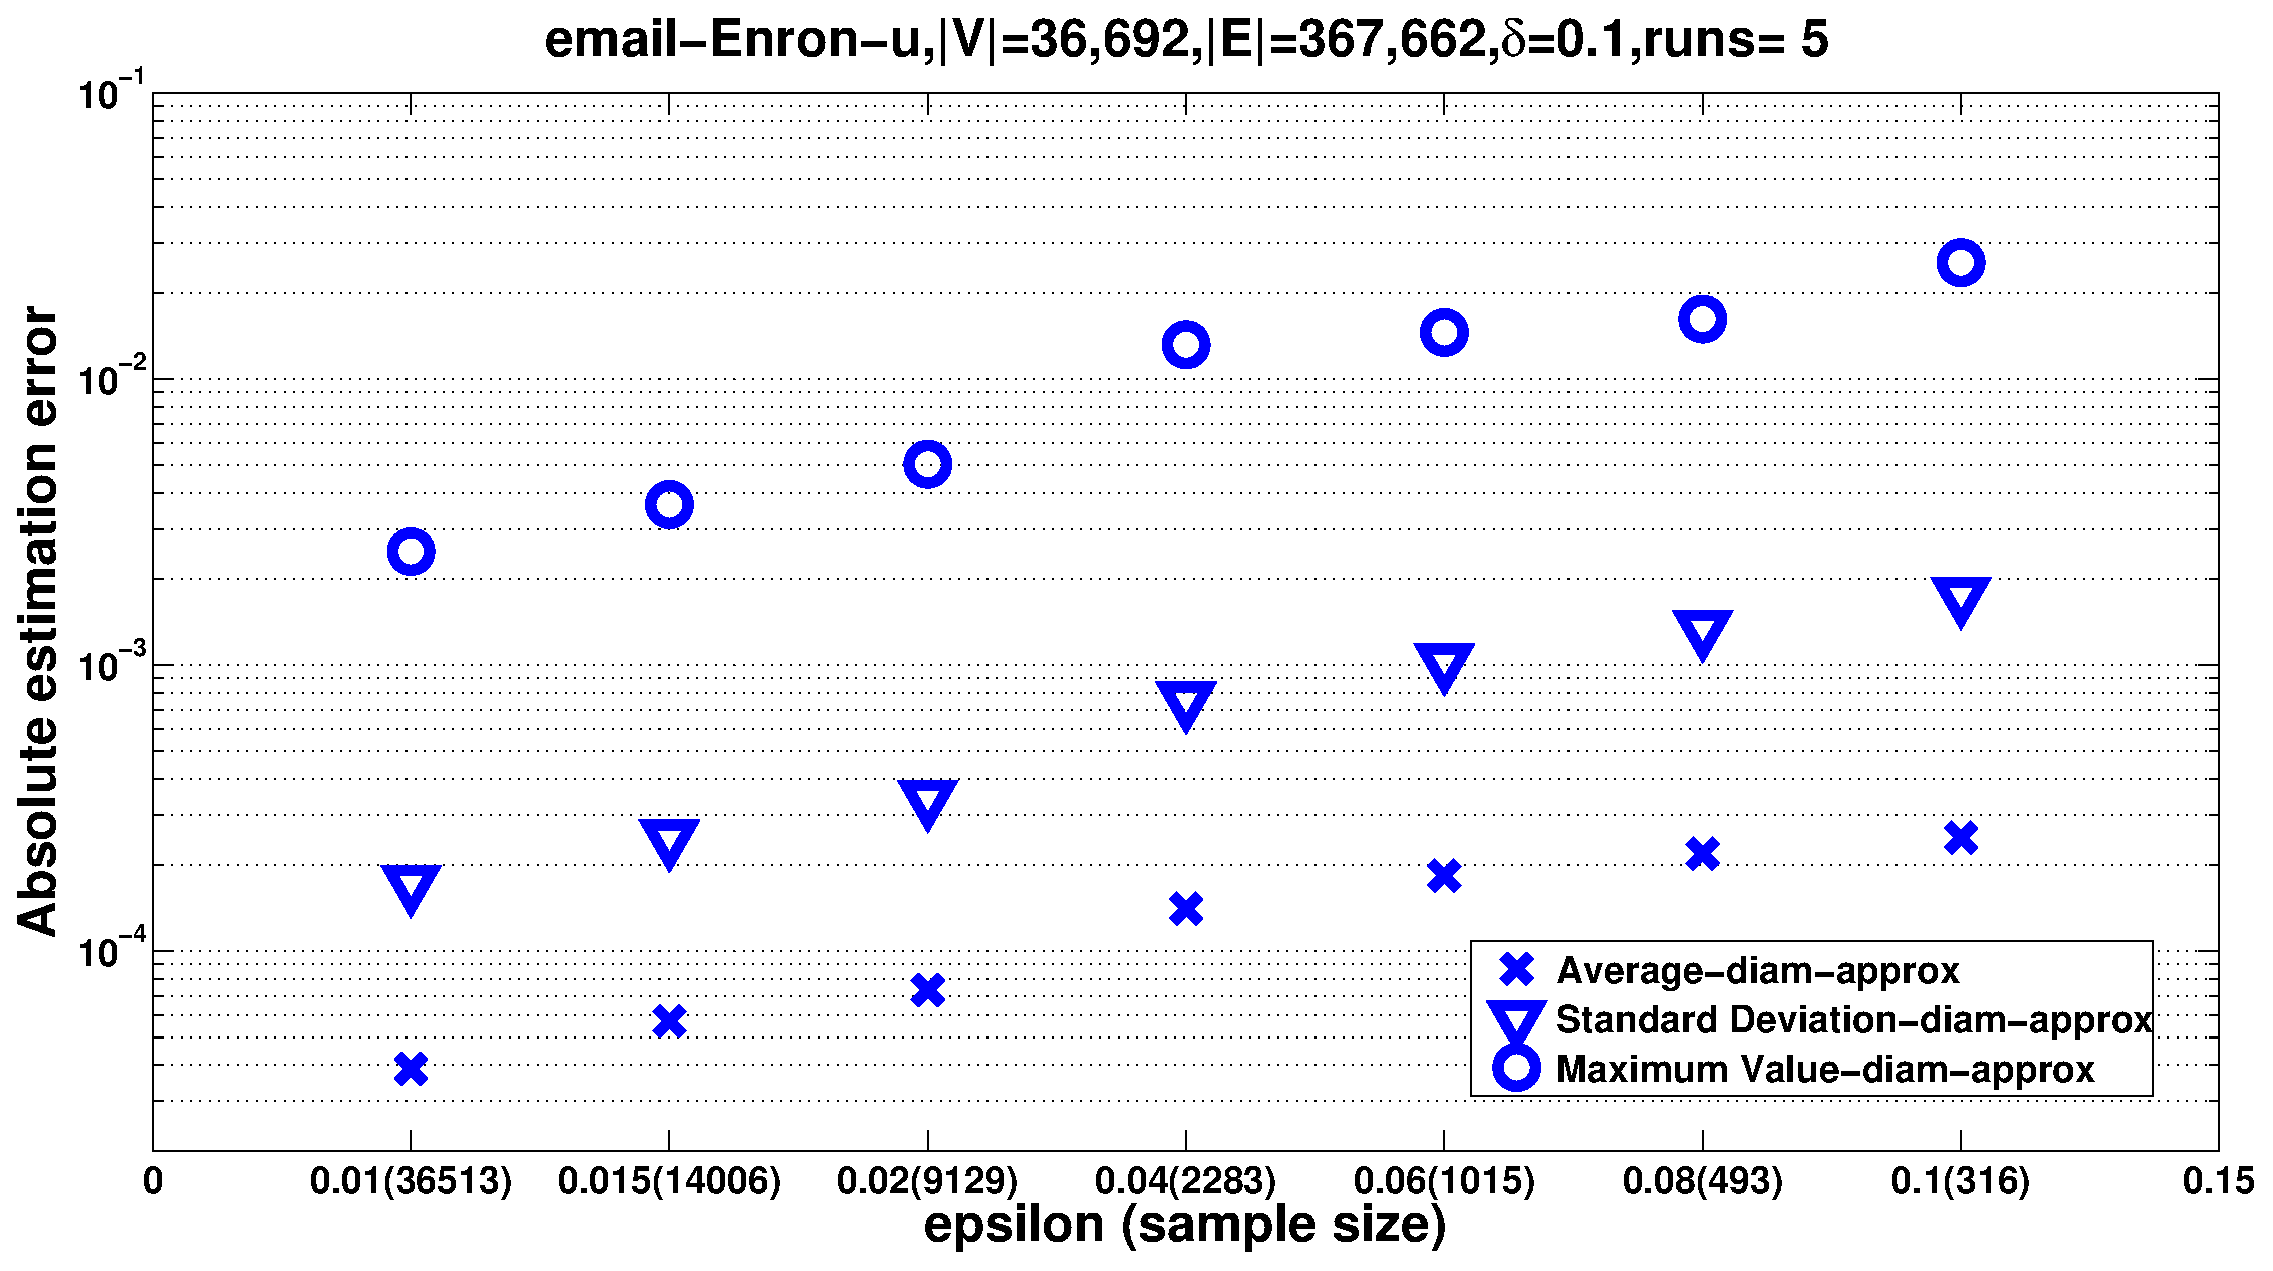
\includegraphics[width=0.7\textwidth,keepaspectratio]{figures/eps/email-Enron-error}
    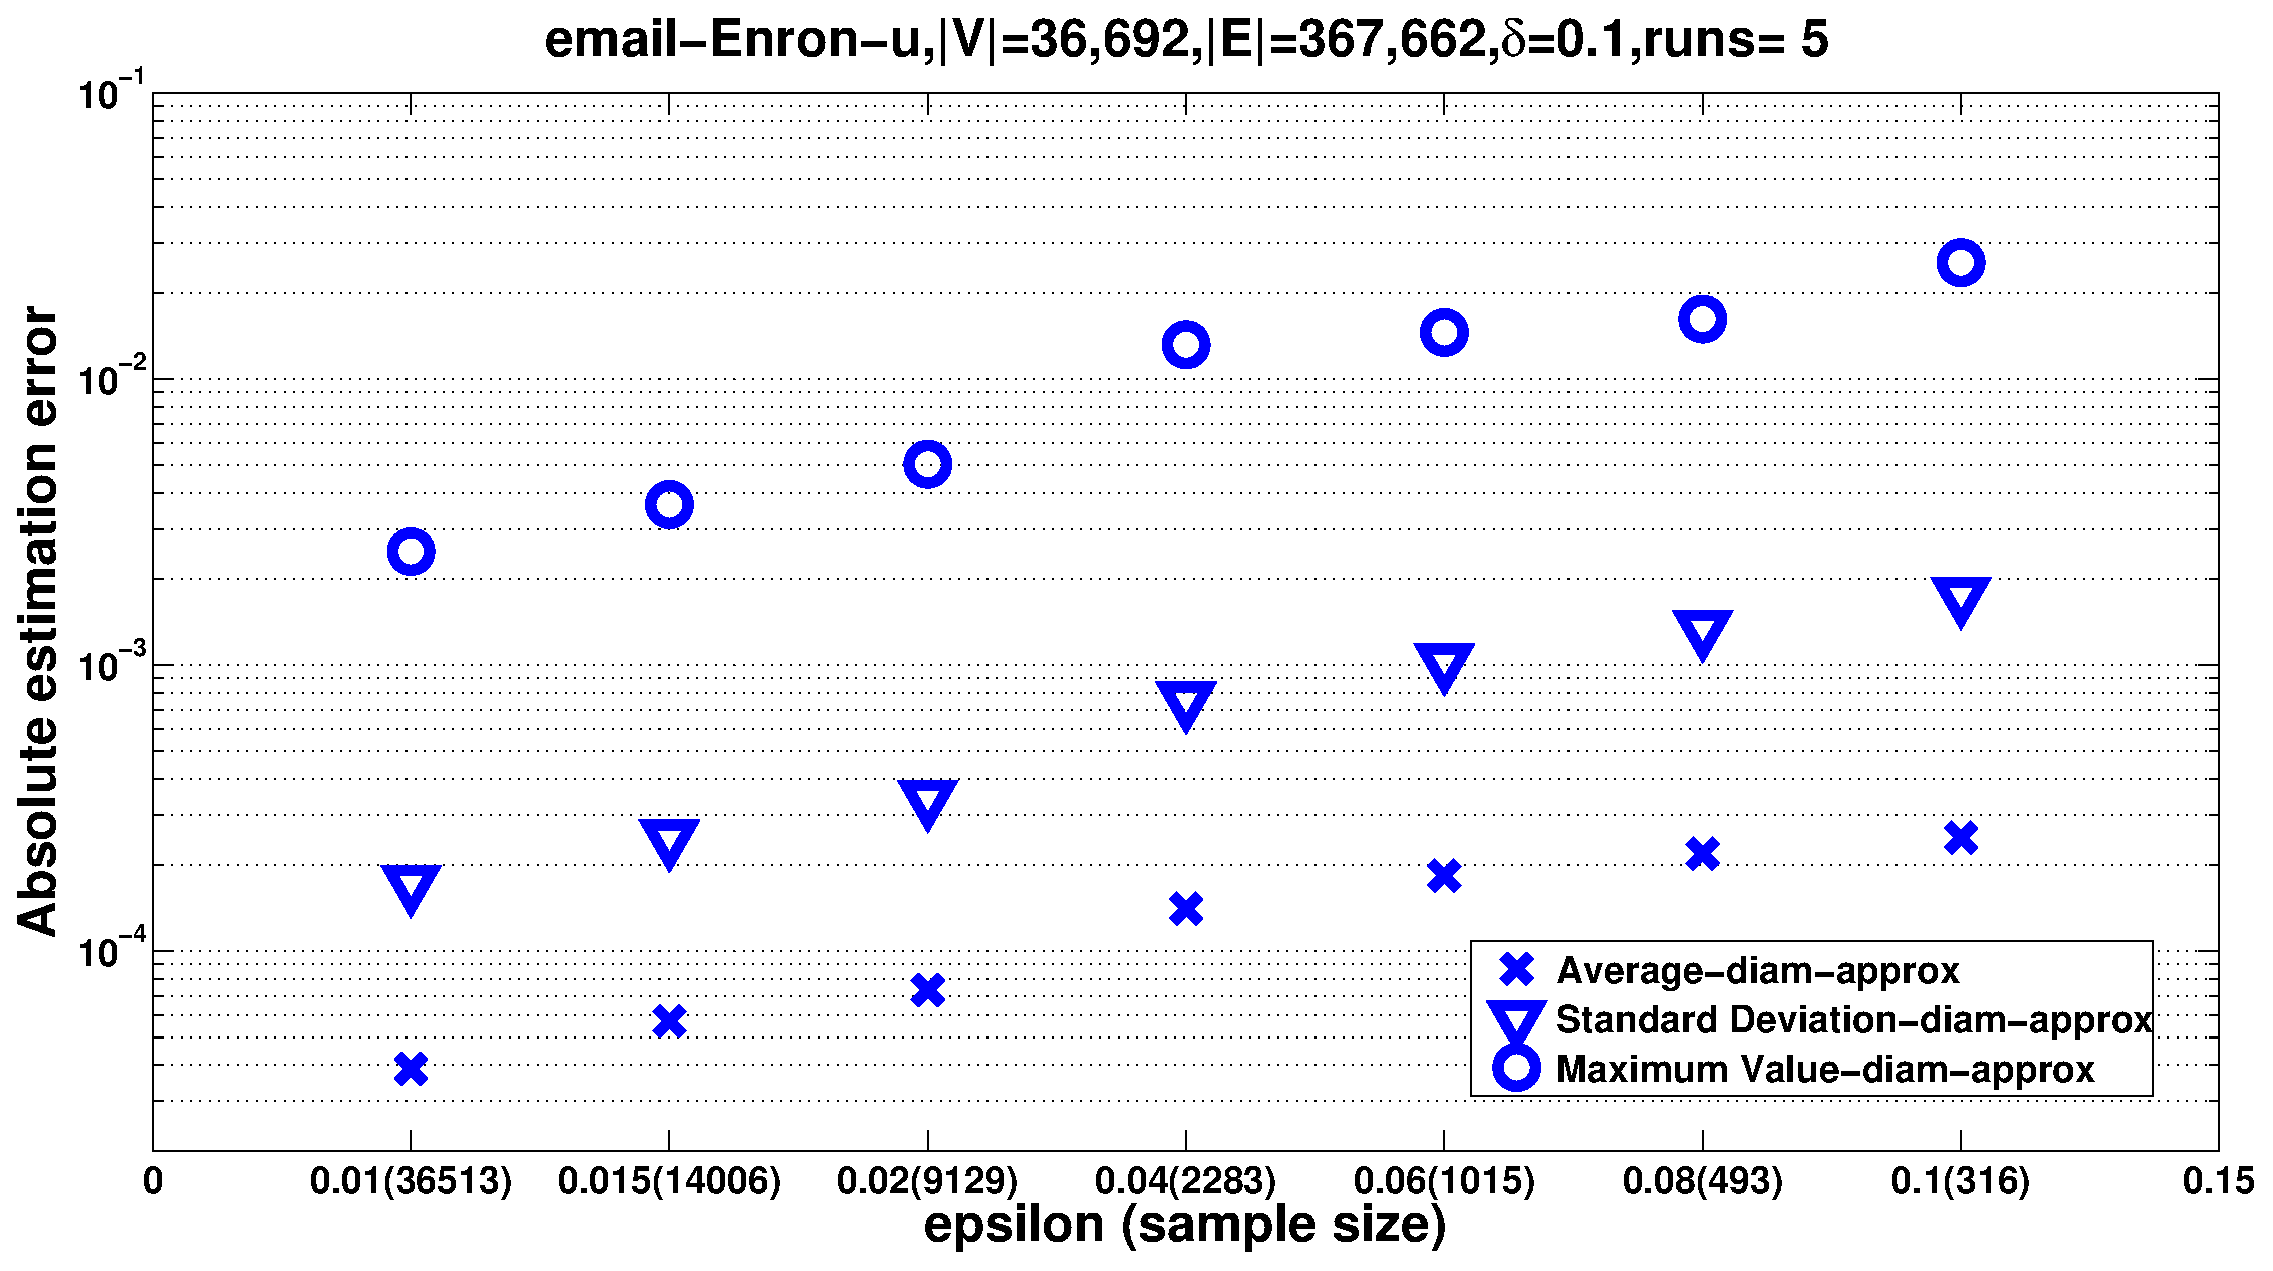
\includegraphics[width=\textwidth,height=0.18\textheight]{figures/eps/email-Enron-error}
    \caption{email-Enron (undirected)}
    \label{fig:email:error}
  \end{subfigure}
  \caption{Betweenness estimation error $|\tilde\betw(v)-\betw(v)|$ evaluation
  for directed and undirected graphs as function of $\varepsilon$. The reported
  quantities are: average error, maximum error, and the sum between average and
  standard deviation. For directed graphs, two versions of these quantities are
  reported, one for runs of the algorithm using the exact vertex diameter, and
  one for runs using an upper bound to it. For undirected graph we report the
  quantities for runs that used the 2-approximation to the vertex diameter.}\label{fig:error}
\end{figure*}

\begin{figure*}[htbp]
  \centering
  \begin{subfigure}[b]{1\textwidth}
    \includegraphics[width=1\textwidth,height=0.19\textheight]{figures/eps/p2p-Gnutella30-time}
    \caption{p2p-Gnutella30 (directed)}
    \label{fig:gnutella:time}
  \end{subfigure}
  %\ifproof
  %\hfill

  \begin{subfigure}[b]{1\textwidth}
    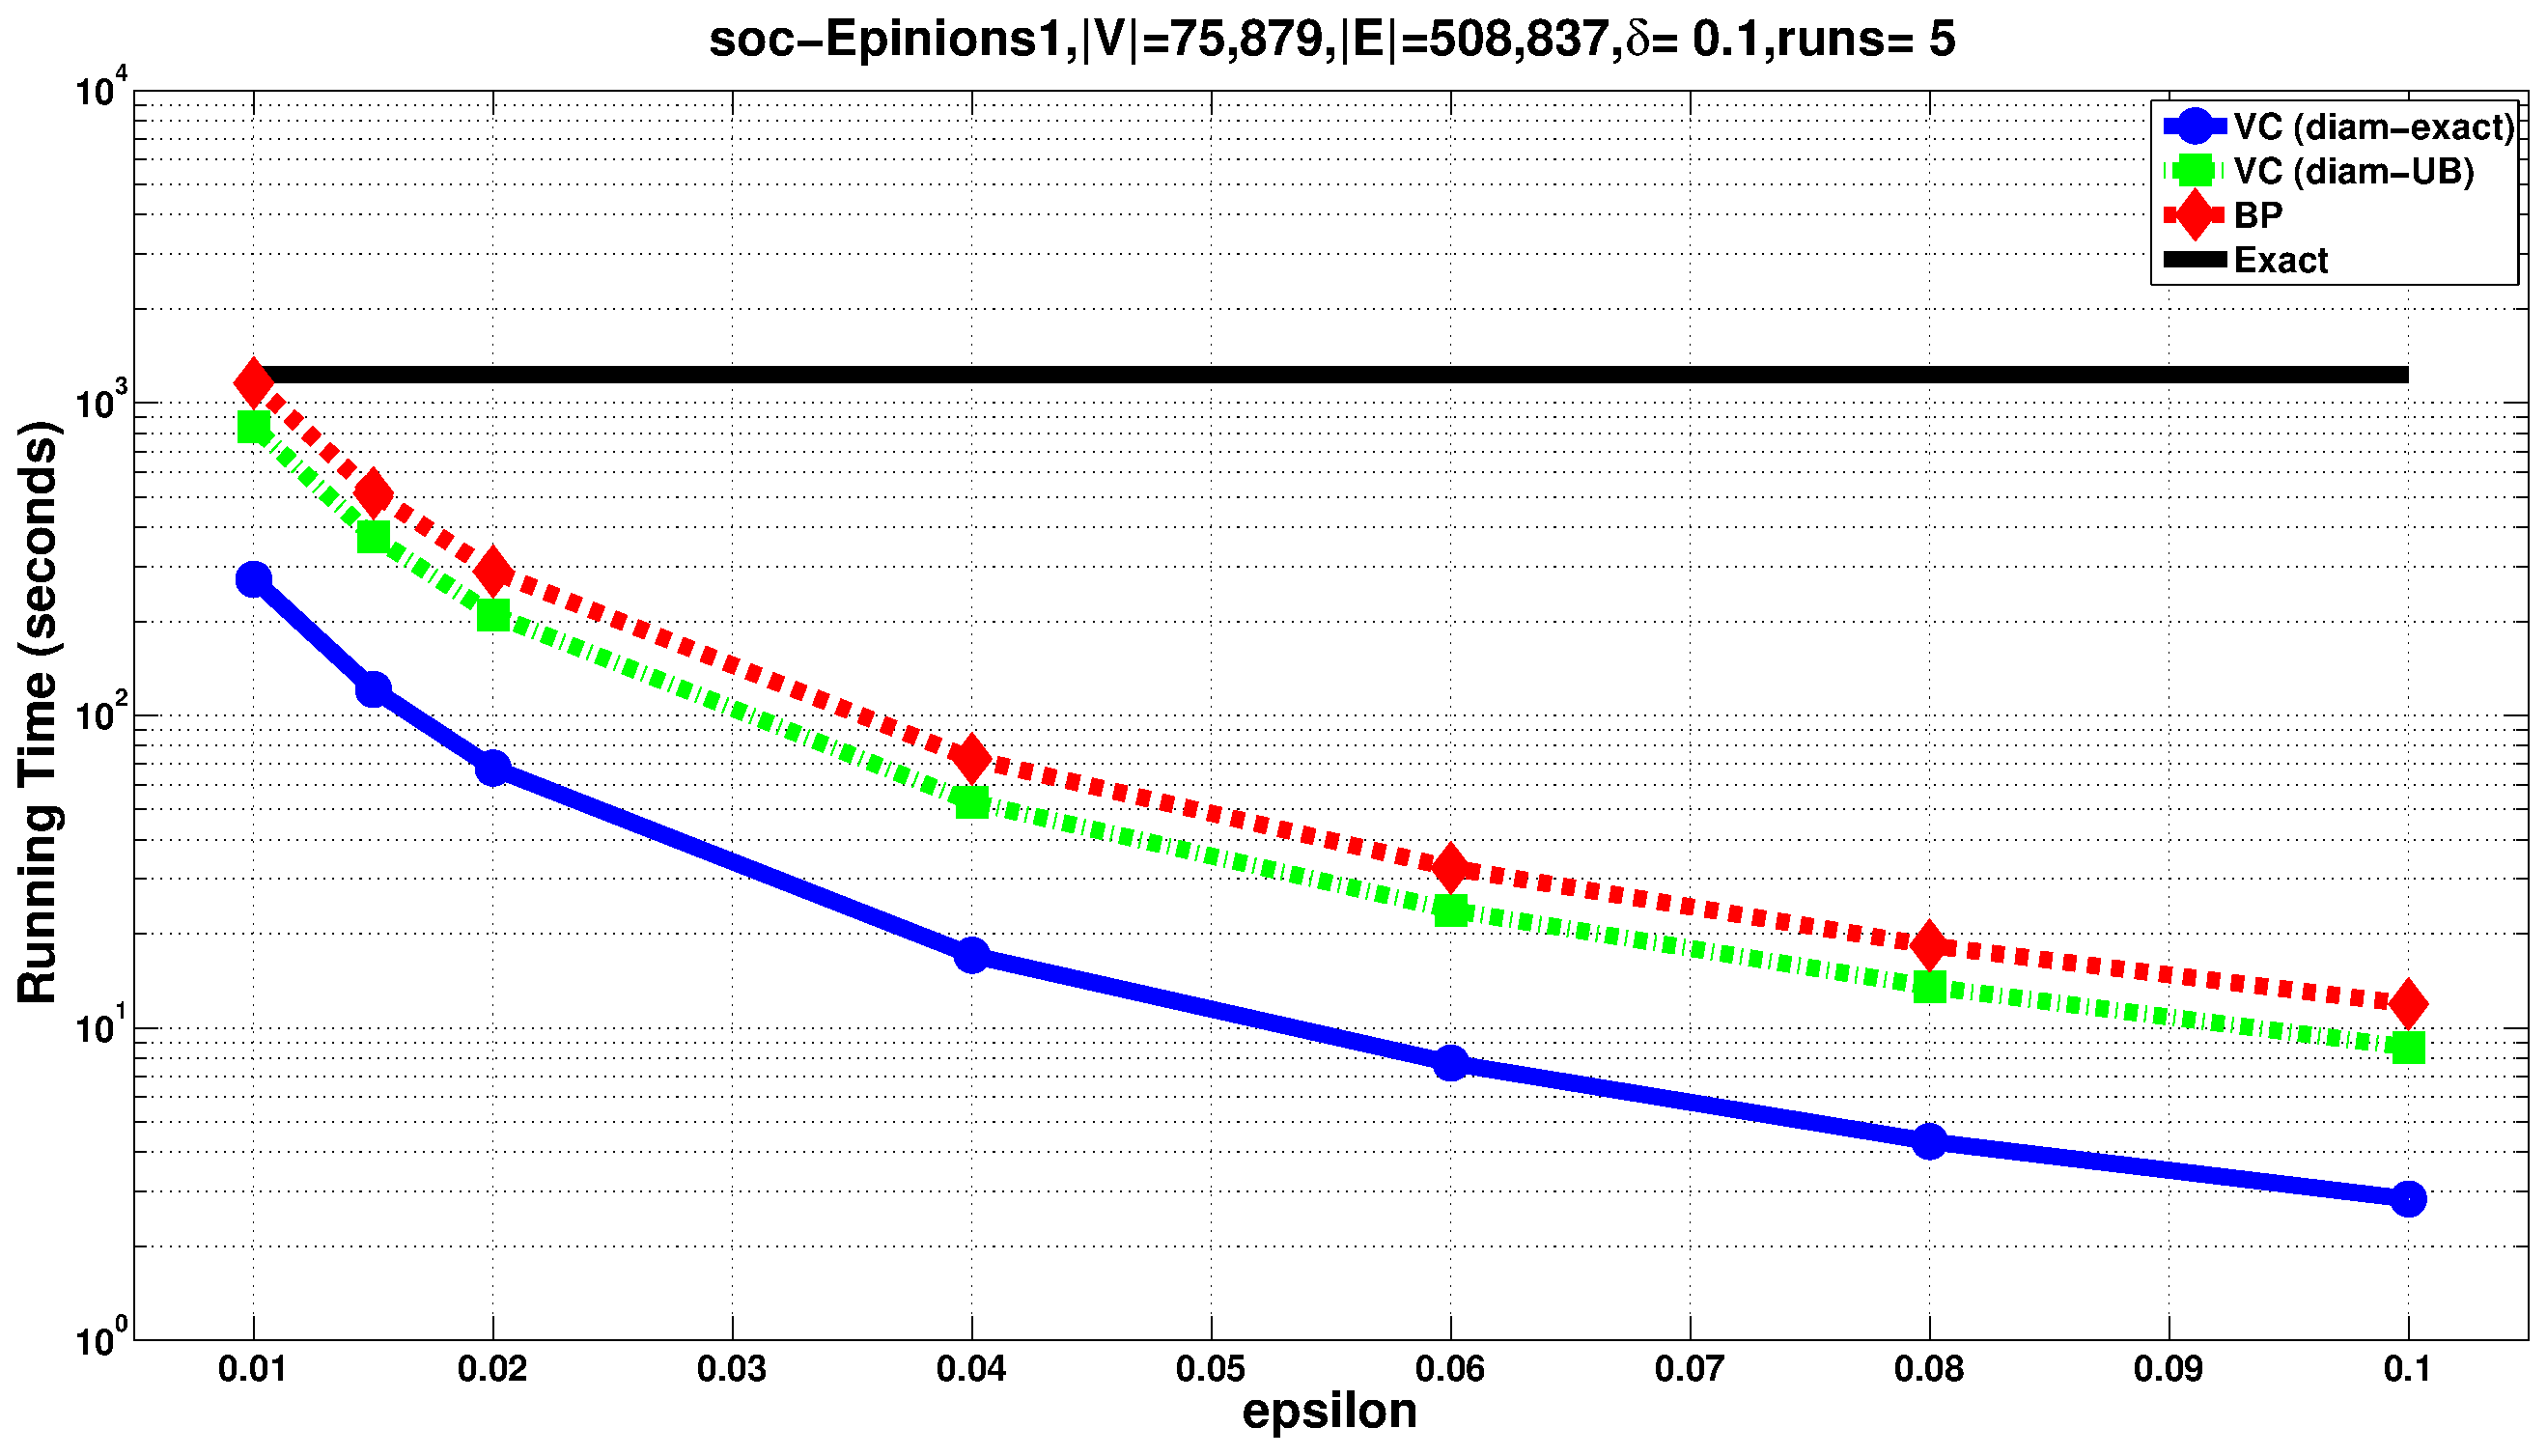
\includegraphics[width=1\textwidth,height=0.19\textheight]{figures/eps/soc-Epinions1-time}
    \caption{soc-Epinions1 (directed)}
    \label{fig:Epinions:time}
  \end{subfigure}

  \begin{subfigure}[b]{1\textwidth}
    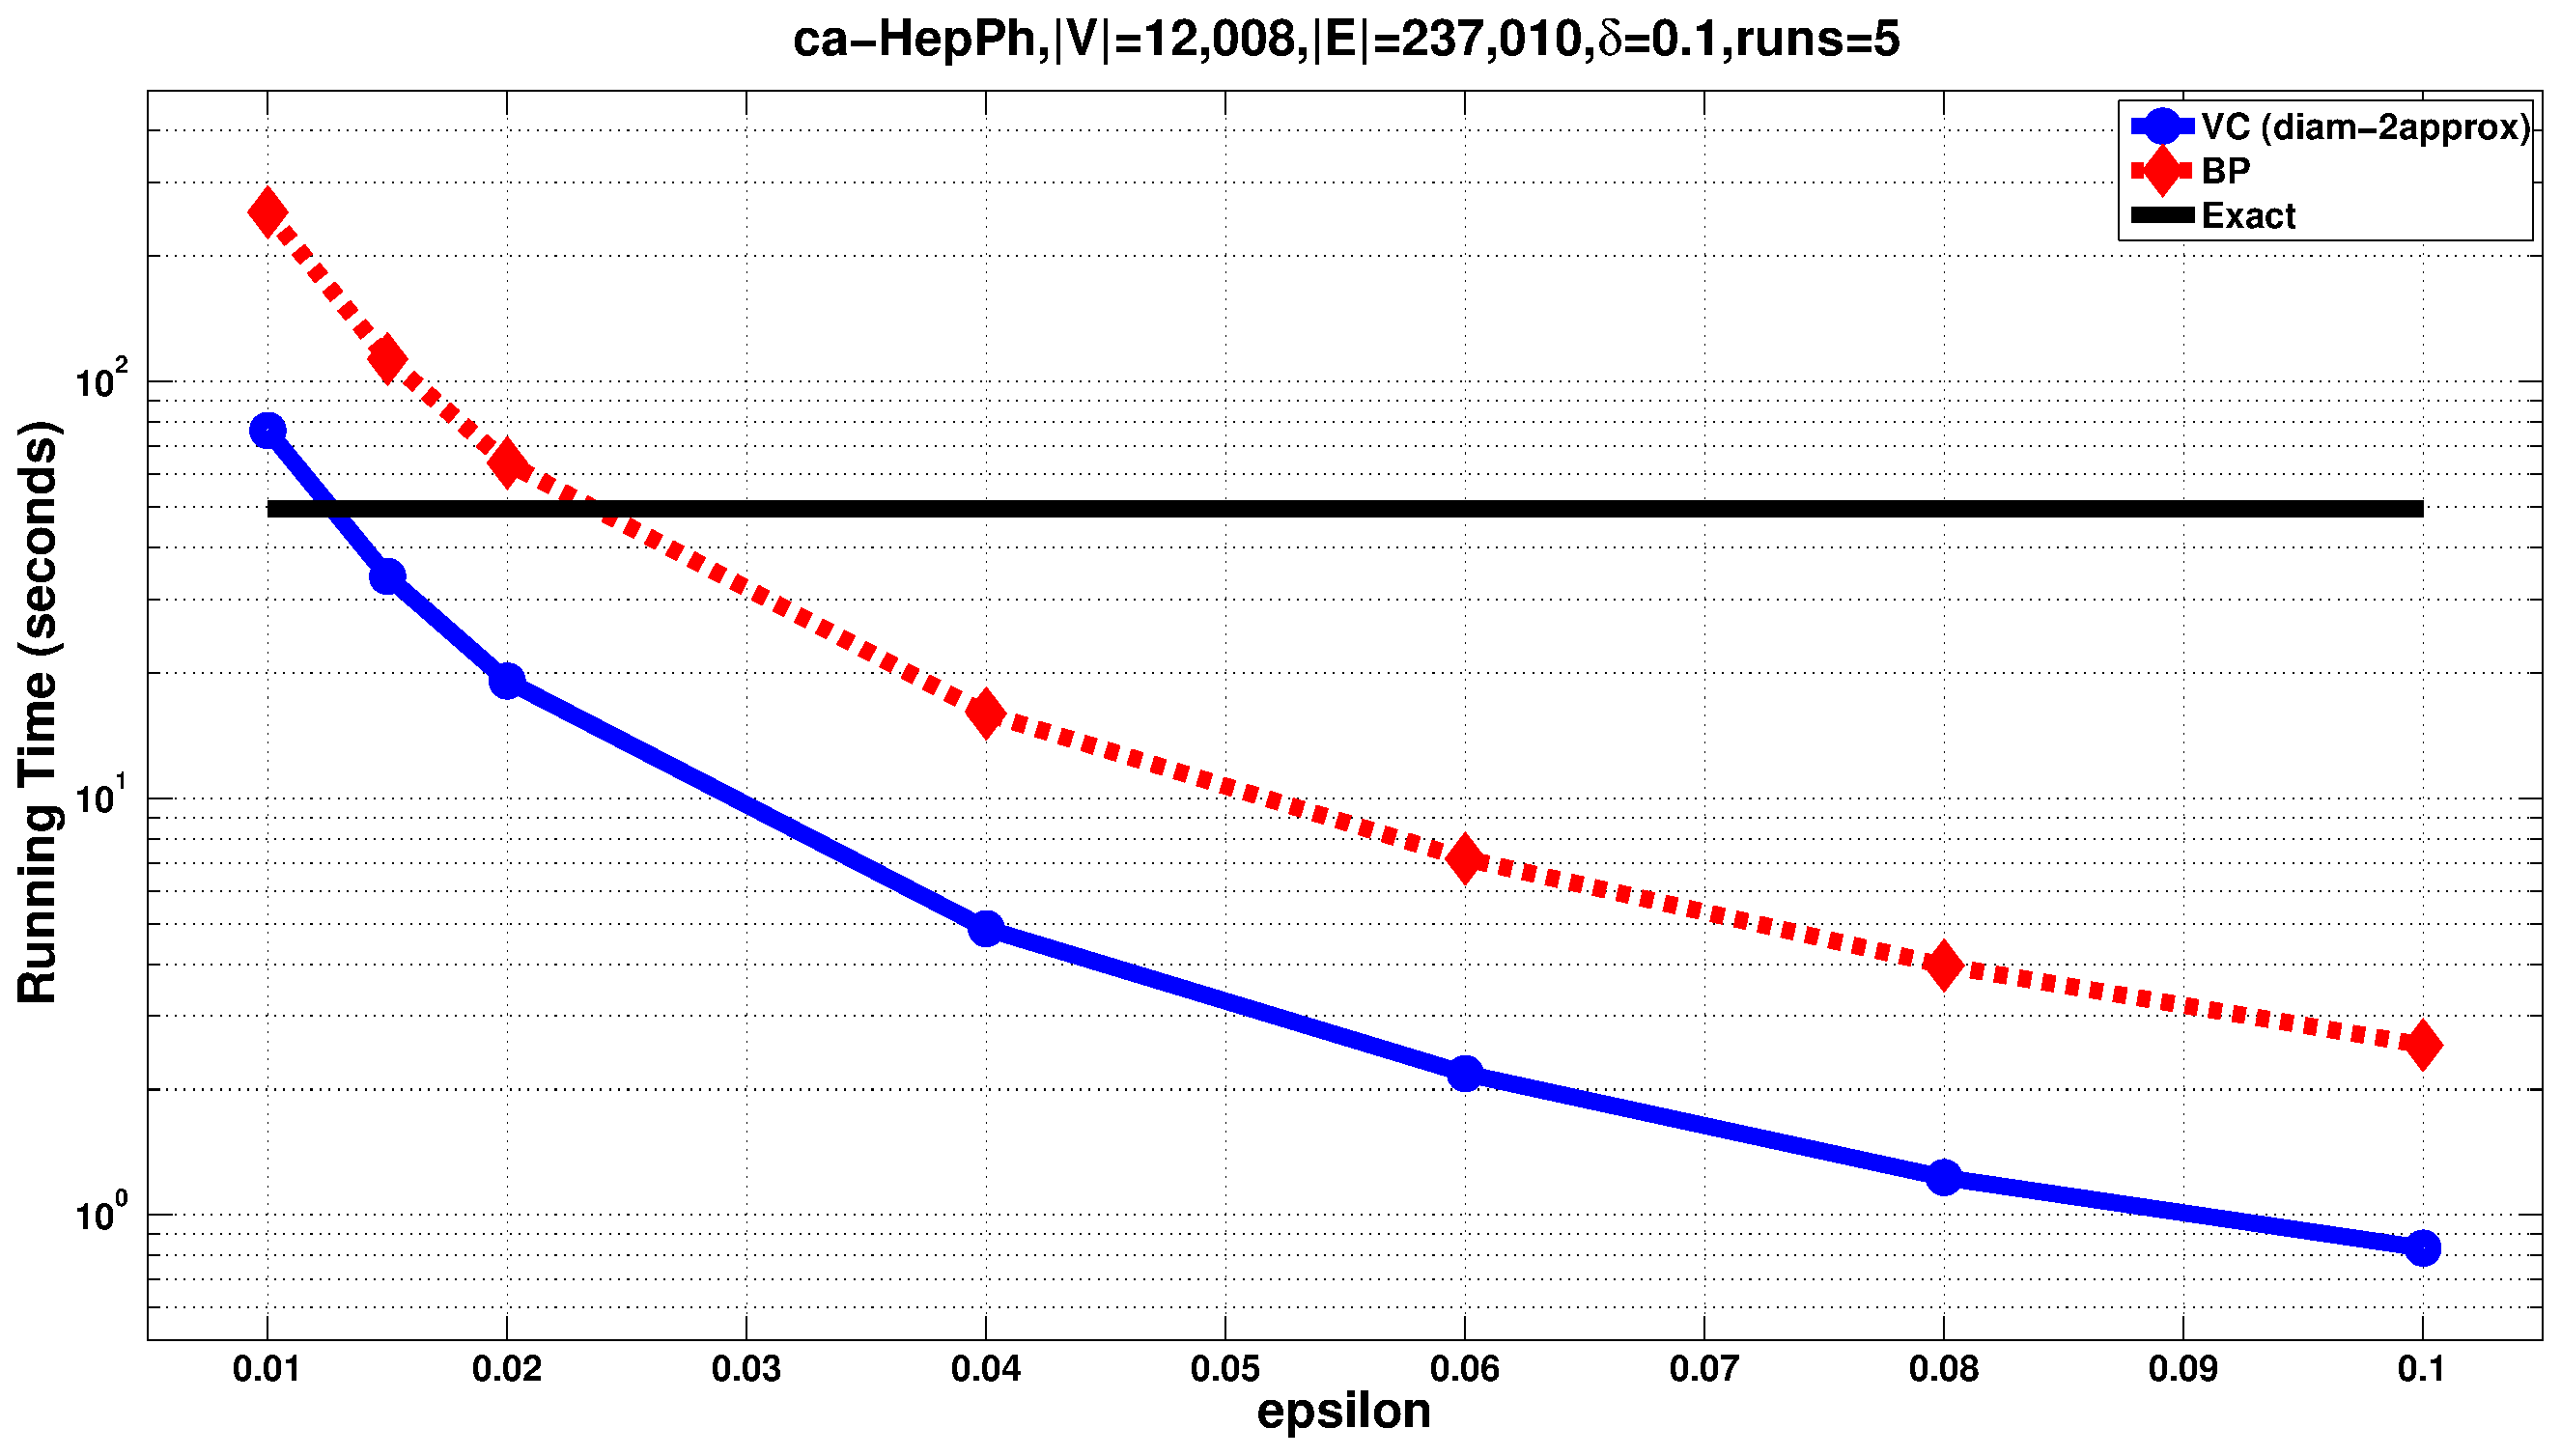
\includegraphics[width=1\textwidth,height=0.19\textheight]{figures/eps/ca-HepPh-time}
    \caption{ca-HepPh (undirected)}
    \label{fig:HepPh:time}
  \end{subfigure}
  %\fi
  %\hfill

  \begin{subfigure}[b]{1\textwidth}
    \includegraphics[width=1\textwidth,height=0.19\textheight]{figures/eps/email-Enron-time}
    \caption{email-Enron (undirected)}
    \label{fig:email:time}
  \end{subfigure}
  \caption{Comparison of the running time (in seconds) between $\mathsf{VC}$,
  $\mathsf{BP}$, and the exact algorithm, as functino of $\varepsilon$. For
  directed graphs, the running time of $\mathsf{VC}$ is reported twice: one for
  runs using the exact vertex diameter, and one for runs using an upper bound to
  this quantity. For undirected graphs we report the running time of
  $\mathsf{VC}$ using the 2-approximation to the diameter.}
  \label{fig:time}
%\begin{minipage}[b]{0.5\linewidth}
%\flushleft
%\includegraphics[width=3.8in, keepaspectratio]{p2p-Gnutella30-time.eps}
%\caption{Running time comparison on p2p-Gnutella30} \label{fig:gnutella:time}
%\end{minipage}%
%\begin{minipage}[b]{0.5\linewidth}
%\centering
%\includegraphics[width=3.8in, keepaspectratio]{email-Enron-time.eps}
%\caption{Running time comparison on email-Enron} \label{fig:email:time}
%\end{minipage}
\end{figure*}
\subsection{Accuracy}\label{sec:accuracy}
Our theoretical results from Sect.~\ref{sec:algo} guarantee that, with probability
at least $1-\delta$, all estimations of the betweenness values for all vertices
in the graph are within $\varepsilon$ for their real value. %, that is
%\[
%\Pr(\exists v\in V \mbox{ s.t. }
%|\betw(v)-\tilde\betw(v)|>\varepsilon)<\delta\enspace.
%\]
We run Algorithm~\ref{alg:algorithm} five times for each graph and each value of
$\varepsilon$ in $\{0.01, 0.015, 0.02, 0.04, 0.06, 0.08, 0.1\}$. The parameter
$\delta$ was fixed to $0.1$ and we used $c=0.5$ in~\eqref{eq:vceapprox} to
compute the sample size, as suggested by~\citet{LofflerP09}. As far as the
\emph{confidence} is concerned, we report that in all the hundreds of runs we
performed, the guarantee on the quality of approximation was \emph{always} satisfied, not just
with probability $1-\delta$ ($=0.9$). We evaluated how good the estimated values
are by computing the average \emph{estimation error} $(\sum_{v\in
V}|\betw(v)-\tilde\betw(v)|)/|V|$ across five runs of our algorithm and taking
the average and the standard deviation of this measure, for different values of
$\varepsilon$. We also compute the maximum error $|\betw(v)-\tilde\betw(v)|$
overall. The results are reported in Fig.~\ref{fig:gnutella:error} for the directed
graph p2p-Gnutella30, %
\ifproof
in Fig.~\ref{fig:HepPh:error} for the undirected graph ca-HepPh, in
Fig.~\ref{fig:Epinions:error} for the undirected graph soc-Epinions1, %
\fi
and in Fig.~\ref{fig:email:error} for the undirected graph
email-Enron. %
\ifproof
\else
Results for other graphs are similar~\citep{RiondatoK13}. %
\fi
It is
evident that the maximum error is an error of magnitude smaller than the
guaranteed value of $\varepsilon$ and that the average error is almost two
orders of magnitude smaller than the guarantees, and the \texttt{Avg+Stddev}
points show that the estimation are quite concentrated around the
average. We can conclude that in practice the algorithm performs even \emph{better
than guaranteed}, achieving higher accuracy and confidence than what the
theoretical analysis indicates. This is due to a number of factors, for example the
fact that we use an \emph{upper bound} to the VC-dimension of the range set and
that the sample size is therefore an upper bound to the one \emph{necessary} to
obtain the desired approximation guarantees.
%Morev the inherent looseness of the formula of the sample size~\eqref{eq:vceapprox}.



\subsection{Runtime}\label{sec:runtime}
We compared the running time of Algorithm~\ref{alg:algorithm} (denoted in the
following as $\mathsf{VC}$ to that of the algorithm presented
by~\citet{JacobKLPT05,BrandesP07,GeisbergerSS08}
(denoted as $\mathsf{BP}$), and to that of the exact
algorithm by~\citet{Brandes01}. As $\mathsf{VC}$ and $\mathsf{BP}$ give the same
guarantees on the accuracy and confidence of the computed estimations, it makes
sense to compare their running times to evaluate which is faster in achieving
the goal. The algorithm proposed by~\citet{GeisbergerSS08}
takes the same time as $\mathsf{BP}$, because it follows the same sampling
approach and only differs in the definiton of the estimator for the betweenness,
so we do not report those.
%as the one
%from~\citep{BrandesP07,JacobKLPT05} and only differs in the definition of the
%estimator for the betweenness of a vertex. Because of this, it takes the same
%amount of time and touches the same number of edges as the one
%from~\citep{BrandesP07}.
%We use two metrics in order to measure the amount of computations that the
%algorithms perform. The first metric is the execution time, or \textit{time}, in
%seconds, the second metric is the number of edges that the algorithm
%touched/traversed, or \textit{touched edges}, during the execution. The number
%of touched edges is a graph theoretic metric \XXX What do you mean by that? that
%does not depend on the specifications of the implementation environment and
%gives a perspective of the amount of work that the algorithm requires. It is
%worth mentioning that we count an edge as many times as it is touched during
%a run of an algorithm, so we might count a single edge more than once.
The algorithms $\mathsf{VC}$ and $\mathsf{BP}$ take parameters $\varepsilon$ and
$\delta$ and compute the sample size accordingly. 
%For our experiments we used
%$\delta=0.1$, while $\varepsilon$ takes value in $\{0.01, 0.015, 0.02, 0.04,
%0.06, 0.08, 0.1\}$.
 We run each experiments five times for each value of $\varepsilon$, and
measured the average running time across the runs.
%as well as the average number of touched edges.  
The results are presented in Figs.~\ref{fig:tables} 
%and~\Cref{fig:gnutella:time,fig:gnutella:edges,fig:email:time,fig:email:edges}.
and~\ref{fig:time}. 
%
In Fig.~\ref{tab:expUndir} we report the minimum and the maximum ratio of the
running time of $\mathsf{BP}$ over $\mathsf{VC}$, taken over the ratios obtained
by running the algorithms with the different values of $\varepsilon$. As it can
be seen from this table our algorithm performs significantly faster, more than
300\%. Similar results are reported for directed graphs in Fig.~\ref{tab:expDir}.
%In~\Cref{tab:expDir} we compare the
%algorithms on a set of directed graphs. As in the case of the undirected graphs,
%we present the minimum and maximum ratios of corresponding measures for the
%different values of $\varepsilon$. 
The diam-UB
and the diam-exact values can be seen as the two extremes for the performance of 
Algorithm~\ref{alg:algorithm} in terms of runtime. In the case of the diam-exact
we have as few samples as possible (for $\mathsf{VC}$) since we use the exact
value of the vertex-diameter, whereas in the case of diam-UB we have as many
samples as possibles because we use the worst case estimation for the
vertex-diameter of the graph.  %(that is when the graph has a hamiltonian path) <= not correct.  
From Fig.~\ref{tab:expUndir} we can see that the value for the
vertex-diameter that we consider in the case of diam-UB $(|V|-2)$ is many orders of
magnitudes greater than the actual value, which translates in a significant
increase of the number of samples. But even in the case of this crude
vertex-diameter approximation (diam-UB), the $\mathsf{VC}$ algorithm performs uniformly faster than
$\mathsf{BP}$. In the case where the exact value of the diameter was used, we
can see that our algorithm computes an estimation of the betweenness that
satisfies the desired accuracy and confidence guarantees \emph{3 to 5 times
faster} than~$\mathsf{BP}$. 
%\XXX-(COMMENT ON THE RELATION TOPOLOGY-SPEED) \MR I have no idea what you meant by that. 
 In Fig.~\ref{fig:gnutella:time} we study
the directed graph p2p-Gnutella30 and we present the measurements of
the average running time of the algorithms for different values of
$\varepsilon$, using the exact algorithm by~\citet{Brandes01} as baseline. The
$\mathsf{VC}$ algorithm requires significantly less time than the $\mathsf{BP}$
algorithm. The figure also shows that there are values of $\varepsilon$ for
which $\mathsf{BP}$ takes more time than the exact algorithm, because the
resulting sample size is larger than the graph size. Given that $\mathsf{VC}$
uses fewer samples and does fewer operations per sample, it can be used with
lower $\varepsilon$ than $\mathsf{BP}$, while still saving time compared to the
exact computation. Figure~\ref{fig:email:time} shows the average running time of the
algorithms for the undirected graph email-Enron. The behavior is  similar to
that for the undirected case. %In this case our
%algorithm not only performs better but also \emph{scales} better than the one
%from~\citep{BrandesP07} \XXX WHAT DO YOU MEAN SCALES BETTER?. 
%For the computation of the sample size we use the 2-approximation algorithm
%which is enough since what we really use for the computation of sample size is
%the logarithm of the diameter. 
%In~\Cref{fig:gnutella:edges,fig:email:edges}, we study the average number of
%touched edges for the case of the directed graph \texttt{p2p-Gnutella30} and of
%the undirected graph \texttt{email-Enron} respectively. It is evident that again
%our algorithm outperforms $\mathsf{BP}$. 
%From the above Figures and Tables we see that for the tested values of
%$\varepsilon$, the proposed algorithm is faster (at least 3x speedup in case of
%exact diameter on the tested graphs). 
 Algorithm~\ref{alg:algorithm} is faster than $\mathsf{BP}$ for two reasons, both
 originating from from our use of results from the VC-dimension theory:
 \emph{1)} we use a significantly smaller amount of samples anda \emph{2)}
 $\mathsf{VC}$ performs the same amount of computations \emph{per sample} as
 $\mathsf{BP}$ only in the worst case. Indeed our algorithm needs only to find
 the shortest path between a sampled pair of vertices, whereas the algorithms
from~\citep{GeisbergerSS08,BrandesP07} need to compute the shortest paths
between a sampled source and all the other vertices. Since the running time of
the algorithms is directly proportional to the number of edges touched during
the shortest path computation, the use of bidirectional A\textsuperscript{*}
search~\citep{Pohl69,KaindlK97} can help in lowering the number of touched edges
for $\mathsf{VC}$ and therefore the runtime of our algorithm ($\mathsf{BP}$
would not benefit from this improvement). %
\ifdmkd
\else
We plan to explore this in future work.
\fi

\begin{figure}[htb]
  \centering
  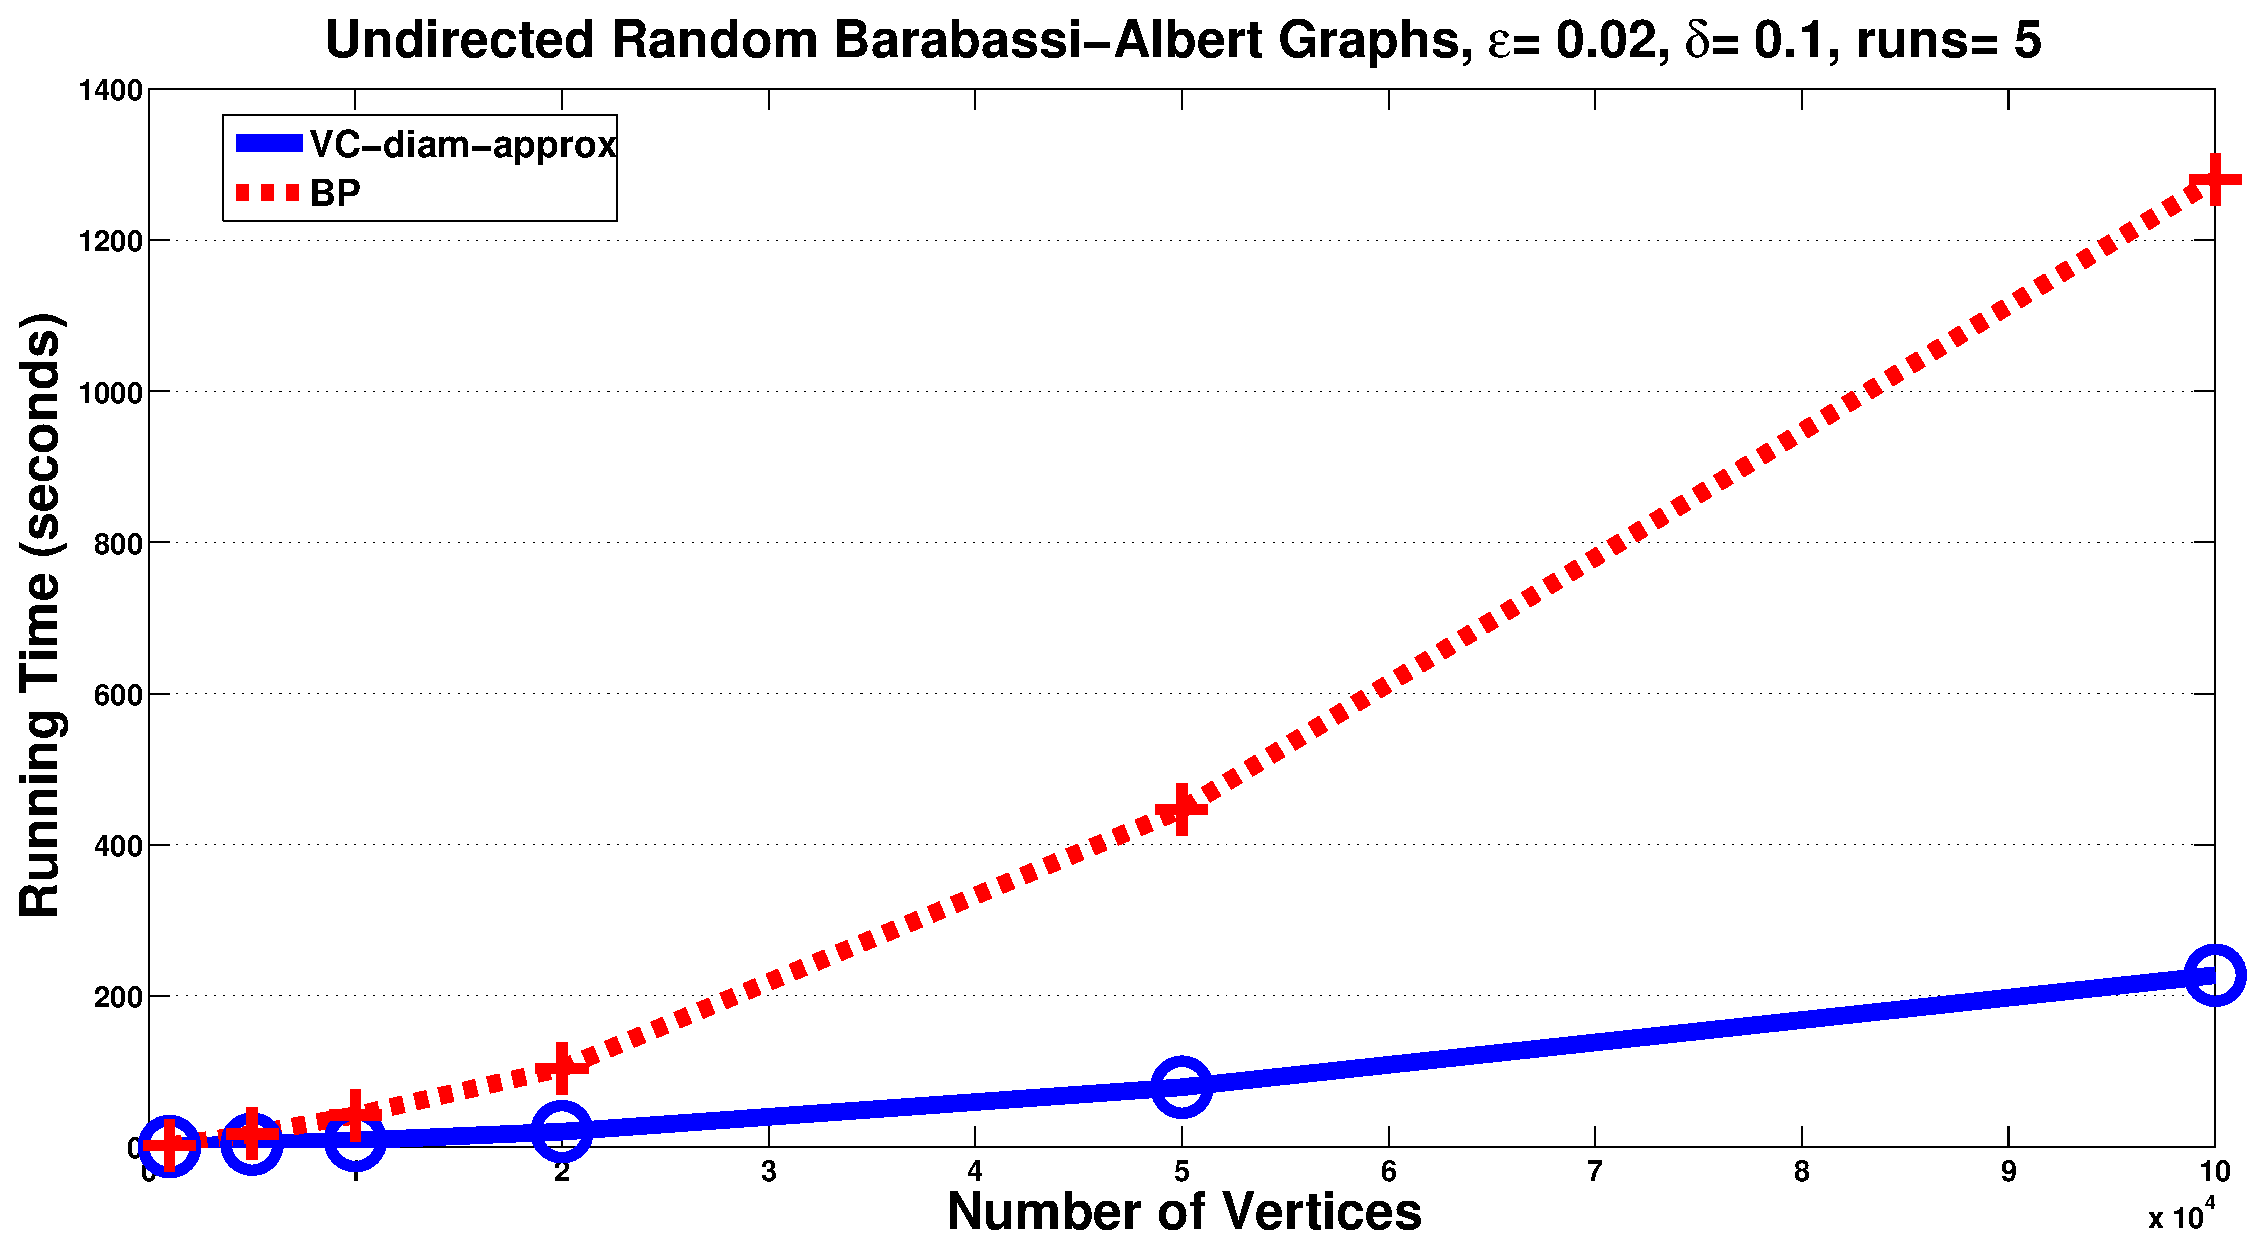
\includegraphics[width=1\textwidth,keepaspectratio]{figures/eps/random-time}
  \caption{Comparison of scalability (running time in seconds) between
  	  $\mathsf{VC}$ and $\mathsf{BP}$ on random undirected
  	  Barab\'asi-Albert~\citep{BarabasiA99} graphs, as function of the number of
	  vertices in the graph. We report the running time for runs of $\mathsf{VC}$ using
	  the 2-approximation to the vertex diameter.}
  \label{fig:random:time}
\end{figure}
\subsection{Scalability}\label{sec:scalability}
In Sect.~\ref{sec:discussion} we argued about the reasons why
Algorithm~\ref{alg:algorithm} is more scalable than $\mathsf{BP}$, while still
offering the same approximation guarantees. To evaluate our argument in practice, we
created a number of graphs of increasing size (1,000 to 100,000 vertices) using
the Barab\'asi-Albert~\citep{BarabasiA99} and run the algorithms on them,
measuring their running time. We report the results in Fig.~\ref{fig:random:time}.
The most-scalable algorithm would be completely independent from the size
(number of vertices) of the graph, corresponding to a flat (horizontal) line in
the plot. Therefore, the less steep the line, the more independent from the
network size would be the corresponding algorithm. From the figure, we can
confirm that this is the case for $\mathsf{VC}$, which is much more scalable
and independent from the size of the sample than $\mathsf{BP}$. This is very
important, as today's networks are not only huge, but they also grow rapidly,
and algorithms to mine them must scale well with graph size.


\section{Conclusions}\label{sec:concl}
In this work we presented two random-sampling-based algorithms for accurately and
efficiently estimate the betweenness centrality of the (top-$K$) vertices in a
graph, with high probability.
%For very large graphs, exact computation of the
%betweenness centrality is impossible, so one has to resort to an approximation.
Our algorithms take a different approach than previous ones achieving the same
guarantees~\citep{BrandesP07,GeisbergerSS08,JacobKLPT05}. They are based on a
completely novel application of results from VC-dimension theory. We show that
the number of samples needed to approximate the betweenness with the desired
accuracy and confidence does not depend on the number of vertices in the graph,
but rather on a characteristic quantity of the network that we call
\emph{vertex-diameter}. In some cases, the sample size is actually completely
independent from any property graph, which is interesting and unexpected.
Our algorithms perform much less work than previously presented methods offering
the same approximation guarantee. As a consequence, they are much faster and
scalable. These claims were verified during our extensive experimental
evaluation using many real and artificial graphs. In future work we would like
to explore the possibility of using bidirectional A\textsuperscript{*}
search~\citep{Pohl69,KaindlK97} to further speed up our algorithms.  We are also
interested in extending our methods to generalizations of betweenness
centrality~\citep{KourtellisASIT12,DolevEP10} and to other centrality measures. 

\paragraph*{Acknowledgements} We are thankful to Eli Upfal for his guidance and
support throughout this project and to the anonymous reviewers whose comments
helped us improving this work.




%\bibliographystyle{abbrvnat}
%\bibliographystyle{IEEEtranS}
\bibliographystyle{IEEEtranSN}
\bibliography{diamapprox,vcmine,vcgraph,centrality}


\end{document}

